\documentclass[
    % -- opções da classe memoir --
    12pt,                 % tamanho da fonte
    openright,            % capítulos começam em pág ímpar (insere página vazia caso preciso)
    oneside,              % para impressão em um lado. Oposto a twoside, verso e anverso
    a4paper,              % tamanho do papel. 
    % -- opções da classe abntex2 --
    chapter=TITLE,        % títulos de capítulos convertidos em letras maiúsculas
    section=TITLE,        % títulos de seções convertidos em letras maiúsculas
    % -- opções do pacote babel --
    english,              % idioma adicional para hifenização
    brazilian,            % o último idioma é o principal do documento
]{styles/abntex2}


\usepackage[alf,
    %versalete,
    abnt-emphasize = bf, % destaca o titulo da revista ou livro em negrito;
    abnt-etal-list = 3, % trabalhos com mais de 3 autores recebem et al.,;
    %abnt-etal-text = it, % escreve o et al., em italico;
    bibliographystyle = styles/abntex2-alf.bst,
    abnt-repeated-author-omit = no % autores com + de uma entrada recebem '____.'
]{styles/abntex2cite}

\usepackage[utf8]{inputenc}

%\usepackage[dvipsnames]{xcolor}
\usepackage[table,xcdraw,dvipsnames]{xcolor}
%\usepackage{subfigure}   % Pacote para subfiguras
\usepackage{amsmath}
\usepackage{lastpage}
\usepackage{times}
\usepackage{graphicx}
\usepackage{caption}
\usepackage{tocloft}
\usepackage{tabularx}
\usepackage{booktabs}
\usepackage{enumitem}
\usepackage{dirtytalk}
\usepackage{tikz}
\usetikzlibrary{tikzmark}
%\usepackage{array} 
\usepackage{multirow}
\usepackage{threeparttable} % to use table notes

\usepackage{caption}
\usepackage{textcomp}


%%%%%%%%%%%%%%%%%%%%%%%%%%%%%%%%%%%%%%%%%%%%%%%%%%%%%%%%%%%%%%%%%
%%%%%%%%%%%%%%%%%%%%%%%%%%%%%%%%%%%%%%%%%%%%%%%%%%%%%%%%%%%%%%%%%
%%%%%%%%%%%%%%%%%%%%%%%%%%%%%%%%%%%%%%%%%%%%%%%%%%%%%%%%%%%%%%%%%
\usepackage{listings}
\usepackage{xcolor}

%New colors defined below
\definecolor{codegreen}{rgb}{0,0.6,0}
\definecolor{codegray}{rgb}{0.5,0.5,0.5}
\definecolor{codepurple}{rgb}{0.58,0,0.82}
\definecolor{backcolour}{rgb}{0.95,0.95,0.92}

% Code listing style named "mystyle"
\lstdefinestyle{mystyle}{
    backgroundcolor=\color{backcolour}, commentstyle=\color{codegreen},
    keywordstyle=\color{magenta},
    numberstyle=\tiny\color{codegray},
    stringstyle=\color{codepurple},
    basicstyle=\ttfamily\footnotesize,
    breakatwhitespace=false,         
    breaklines=true,                 
    captionpos=b,                    
    keepspaces=true,                 
    numbers=left,                    
    numbersep=5pt,                  
    showspaces=false,                
    showstringspaces=false,
    showtabs=false,                  
    tabsize=2
}

%"mystyle" code listing set
\lstset{style=mystyle}
%%%%%%%%%%%%%%%%%%%%%%%%%%%%%%%%%%%%%%%%%%%%%%%%%%%%%%%%%%%%%%%%%

% Criação do symbol da função sign
\DeclareMathOperator{\sign}{sign}

\newcolumntype{C}[1]{>{\centering\let\newline\\\arraybackslash\hspace{0pt}}m{#1}}
\newcolumntype{L}[1]{>{\RaggedRight\let\newline\\\arraybackslash\hspace{0pt}}m{#1}}

% Alinhamento de legenda à esquerda
\captionsetup{justification=raggedright,singlelinecheck=false}

\usepackage{styles/ttc_univali}

\begin{document}
\newcounter{equationCounter}

\pretextual

% Capa e elementos pre-textuais
\begin{Info}
% Universidade
{UNIVERSIDADE DO VALE DO ITAJAÍ}
% Escola
{ESCOLA POLITÉCNICA}
% Curso
{CURSO DE CIÊNCIA DA COMPUTAÇÃO}
% Titulo
{DETECÇÃO DE ERROS EM SISTEMA OPERACIONAL DE TEMPO REAL}
% Autor
{Marcos Augusto Fehlauer Pereira}
% Cidade e Data
{Itajaí (SC), Junho de 2025}
% Nome da Área de concentração
{Sistemas Operacionais}
% Orientador(a)
{Felipe Viel, MSc.}
% Coorientador(a) <Nome do Coorientador(a)>, <Titulação> %%%%%%%% Se não tiver coorientador deixe vazio

\end{Info}

%\begin{Dedicatoria}
% Dedicatória
% \end{Dedicatoria}

% \begin{Agradecimentos}
% Agradeço a todos.
% \end{Agradecimentos}

% \begin{Epigrafe}
% Epígrafe
% \end{Epigrafe}

\begin{Resumo}
Sistemas embarcados são sistemas especializados tipicamente encontrados como um componente lógico de um dispositivo maior, estes sistemas utilizam-se com frequência um tipo especializado de sistema operacional: Sistemas operacionais de tempo real, que permitem que múltiplas tarefas executem de forma concorrente. Em diversas situações é necessário que esses dispositivos operem em condições adversas (como radiação ionizante e interferência eletromagnética) que alteram seu comportamento esperado e degradam sua qualidade de serviço, para operar dentro de tais condições, técnicas de tolerância à falhas são aplicadas, que visam permitir a operação razoável do sistema mesmo na presença de falhas. Para viabilizar tolerância à falhas é possível utilizar de diversos mecanismos, dentre eles, aqueles que operam em conjunto com o escalonador do sistema operacional de tempo real podem permitir um grau de resiliência maior enquanto visando reduzir a ociosidade dos núcleos da máquina. Este trabalho visa explorar e aplicar técnicas de tolerância e detecção de falhas (Redundância Modular, Reexecução, Heartbeat Signal, CRCs e Asserts) com uma interface voltada ao escalonador do sistema operacional, com o objetivo de fornecer uma análise dos custos e vantagens associados à cada combinação de técnicas.

\textbf{Palavras-Chave}: Sistemas Embarcados. Sistemas Operacionais. Tolerância a Falhas. FreeRTOS. Escalonador.

\end{Resumo}

\begin{Abstract}

\textit{Embedded Systems are specialized systems that are typically found as a logical component of a greater device, these systems are frequently equipped with a special kind of operating system: a Real Time Operating System, that allow for multiple tasks to be executed concurrently. In many situations, it is required that such devices operate in adverse or volatile conditions (e.g. ionizing radiation and electromagnetic interference) that alter its behavior, causing a degradation in its quality of service. Thus, to be able to operate within these contexts, fault tolerance techniques are applied, with the goal of allowing reasonable system operation even within the presence of faults. Many mechanisms may be used to achieve fault tolerance, among them, there are those that operate in conjunction with the real time operating system's scheduler to offer a greater degree of reliability while also decreasing idle time of them machine's cores. This work shall explore and apply techniques of fault tolerance (Modular Redundancy, Re-execution, Heartbeat Signal and Asserts) that have an interface focused on the scheduler's capabilities, with the main objective of providing an analysis over the tradeoffs attached to permutations of those techniques.}

\textit{\textbf{Keywords}: Embedded Systems. Operating Systems. Fault Tolerance. FreeRTOS. Scheduler.}

\end{Abstract}

 \clearpage
% ---
% inserir lista de ilustrações
% ---
\pdfbookmark[0]{\listfigurename}{lof}
\listoffigures*
\cleardoublepage
% ---

% ---
% inserir lista de tabelas
% ---
% \pdfbookmark[0]{\listtablename}{lot}
% \listoftables*
% \cleardoublepage
% ---

% ---
% inserir lista de quadros
% ---
\pdfbookmark[0]{\listofquadrosname}{loq}
\listofquadros*
\cleardoublepage
% ---
\pdfbookmark[0]{\listofequacaoname}{loe}
\listofequacao*
\cleardoublepage

% ---
% inserir lista de abreviaturas e siglas
% ---
\begin{siglas}
    \item[COTS]  Commercial Off-The-Shelf
    \item[CRC]   Cyclic Redundancy Check
    \item[CPU]   Central Processing Unit
    \item[FT]    Fault Tolerance
    \item[FFT]   Fast Fourier Transform
    \item[GDB]   GNU Debugger
    \item[iFFT]  Inverse Fast Fourier Transform
    \item[IoT]   Internet of Things
    \item[ITAR]  International Traffic in Arms Re-gulations
    \item[iSCSI] Internet Small Computer Systems Interface
    \item[PCB]   Printed Circuit Board
    \item[QEMU]  Quick EMUlator
    \item[RTOS]  Real Time Operating System
    \item[RAMS]  Reliability, Availability, Mantainability, Safety
    \item[SCTP]  Stream Control Transmission Protocol
    \item[TCC]   Trabalho de Conclusão de Curso
\end{siglas}
% ---

% ---
% inserir o sumario
% ---
\pdfbookmark[0]{\contentsname}{toc}
\tableofcontents*
\cleardoublepage
% ---

 \clearpage

\textual % Indica inicio dos elementos textuais
\pagestyle{simple} % remove o cabecalho

\chapter{Introdução}
\label{cap:intro}

A tolerância a falhas (TF) refere-se à capacidade de um sistema computacional de manter sua qualidade do serviço mesmo na presença de estados adversos. Falhas são comumente observadas em sistemas distribuídos, onde os canais de comunicação estão sujeitos a degradação ou inoperabilidade total devido à interferência eletromagnética, falta de energia e eventos climáticos \cite{FaultTolerantSystems}. Sistemas embarcados enfrentam problemas semelhantes ao operar com canais sujeitos a ruído ou instabilidade, mas também podem ter seus dados em memória ou registradores diretamente corrompidos por causas externas, incluindo: radiação ionizante, flutuações repentinas de temperatura ou voltagem, e colisões físicas \cite{DependabilityInEmbeddedSystems}. A presença desses fenômenos exige que os dispositivos estejam adequadamente preparados, especialmente em aplicações críticas que operam em ambientes voláteis e enfrentam consequências potencialmente catastróficas caso ocorra um erro.

Tornar um sistema tolerante à falhas é um problema multi facetado, ambas soluções em hardware e software necessitam ser abordadas para garantir a qualidade de serviço desejada. O escalonador é o componente crucial de um sistema operacional para a execução concorrente de diversas tarefas \cite{OperatingSystemConcepts}. O processo de detecção das falhas e seu custo de tempo de CPU e uso de memória deve ser considerado pois a reação rápida e correta às falhas requer previamente a detecção e elaboração das rotinas de escalonamento de forma adequada \cite{DependabilityInEmbeddedSystems}.

Este trabalho visa portanto fazer uma análise do impacto de diferentes técnicas de tolerância à falhas durante o escalonamento de tarefas e seu impacto na performance de um sistema, para que se possa melhor compreender e evidenciar os custos e benefícios ao tornar um sistema mais resiliente. 

\section{Problematização}

Sistemas embarcados estão presentes em diversos contextos como: exploração espacial, indústria automotiva, tecnologia médica, dispositivos de baixo consumo energético e sistemas distribuídos no contexto IoT. Portanto, entende-se que manter alto grau da qualidade de serviço com o mínimo de degradação de performance e aumento de custo (monetário ou energético), pode prover uma vantagem econômica para fabricantes e provedores assim como um benefício social na maior confiabilidade no caso de aplicações críticas. \cite{DependabilityInEmbeddedSystems}.

Ademais, ocorreu nos últimos anos uma maior adoção de sistemas COTS (Commercial off the shelf), por poderem ser economicamente mais viáveis e fornecerem uma solução "genérica" para problemas que anteriormente necessitariam de hardware especializado \cite{CyberSecSpaceCOTS}. E mesmo caso pretenda-se utilizar um design especializado para o produto, estes sistemas são úteis para a fase de prototipação e validação do projeto, dado sua facilidade de acesso e flexibilidade.

Um outro fator que influencia na adoção do uso de COTS para certas aplicações que necessitam de tolerância à falhas são as regulações ITAR (International Traffic in Arms Regulations) imposta pelos Estados Unidos que restringe a exportação de diversos tipos de tecnologia de cunho potencialmente militar. Neste caso, o impedimento da exportação certos tipos  tecnologias de PCBs e firmware aumenta mais ainda a necessidade de compradores de outros países adquirirem alternativas comerciais mais comuns que já são complacentes com a regulação \cite{ITARPCBCompliance}.

O custo de utilizar técnicas de tolerância é sensível ao contexto da aplicação e ao nível de tolerância desejado, e no caso dos sistemas COTS, técnicas robustas de resiliência em hardware nem sempre estão disponíveis, sendo necessário delegar esta funcionalidade para a aplicação. É necessário escolher a técnica de tolerância mais adequada de uma multidão de técnicas. Para que a escolha seja informada, é essencial que as trocas em termos de performance e grau de confiabilidade adquiridos sejam compreendidos para minimizar o custo de manter uma qualidade de serviço desejada.

\subsection{Solução Proposta}

Implementar e comparar técnicas de escalonamento com detecção de erros, com o objetivo de esclarecer o impacto de performance em relação ao ganho de dependabilidade do sistema, particularmente no contexto de sistemas com restrição \textit{Hard Real Time}, pois se uma técnica é capaz de satisfazer o critério de tempo real mais rígido, também poderá ser usada em contextos com critério temporal mais relaxado.

\section{Objetivos}

Esta seção formaliza os objetivos do trabalho, conforme descrito a seguir.

\bigskip
\subsection{Objetivo Geral}

Analisar o impacto de técnicas de tolerância à falhas em software num sistema operacional de tempo real.

\bigskip
\subsection{Objetivos Específicos}

\begin{enumerate}
    \item Selecionar técnicas de tolerância à falhas em software
    \item Implementar técnicas escolhidas com uma interface para uso
    \item Realizar testes com de injeção de falhas e coletar métricas de performance das técnicas
    \item Produzir uma análise comparativa das técnicas, seus custos e eficácia
\end{enumerate}

\section{Metodologia}

O objetivo do trabalho é descritivo e exploratório, as métricas coletadas são de caráter quantitativo e conclusões e observações derivadas do trabalho serão realizadas de maneira indutiva baseadas nas métricas de performance coletadas e comparadas.

Foi realizado uma pesquisa bibliográfica para a fundamentação e escolha das técnicas e dos materiais do trabalho, sendo esta primariamente focada em autores com obras associadas ao tema de tolerância assim como temas adjacentes relevantes como sistemas operacionais e interface hardware-software.

Após isso será realizado uma implementação e testes das técnicas escolhidas para validação, e uma campanha de injeção de falhas será realizada em um microcontrolador para a coleta final das métricas no \autoref{cap:proj}.

\section{Estrutura do Trabalho}

No \autoref{cap:fund} serão explorados os tópicos centrais que constituem a premissa do trabalho, primariamente conceitos de detecção de falhas e escalonamento nos sistemas operacionais. Sistemas operacionais são um tópico particularmente vasto, portanto sua abordagem será focada apenas nos aspectos mais essenciais para o trabalho. No \autoref{cap:proj} é definido o projeto e o plano de verificação para a implementação e análise das técnicas descritas. No \autoref{cap:consid} é realizado uma recapitulação do que foi abordado no trabalho e o que se espera ao final de sua conclusão.


 \clearpage
\chapter{Fundamentação Teórica}
\label{cap:fund}

\section{Definições Principais}

Para melhor esclarecer os assuntos abordados, é importante que seja primeiramente definido alguns dos termos centrais para a fundamentação do trabalho.

\subsection{Qualidade de Serviço}

Qualidade de serviço é uma métrica sistêmica que sumariza o quão bem o sistema provisiona suas funcionalidades em um determinado momento. É possível definir e modelar essa métrica de diversas maneiras, mas para os propósitos deste trabalho, será utilizada uma definição simples que resume a funcionalidade geral numa escala de 0 a 1.

A qualidade de serviço $Q$ do sistema pode ser aproximada pela média ponderada de seus serviços $S_0 ... S_n$ com os pesos de seus fatores de contribuição para a qualidade total $q_0 ... q_n$ \cite{SchedAndOptOfDistributedFT}.

\begin{equation}
    Q = \frac{ \sum^{i = 0}_{n} S_i q_i }{ \sum^{i = 0}_{n} q_i}
\end{equation}
\addEquacao{Qualidade de Serviço}{1}

\subsection{Falhas}

De acordo com a definição de anormalidades de software da IEEE: um erro (\textit{error}) é a diferença entre um valor esperado e o valor obtido. Um defeito (\textit{fault}) é um estado irregular do sistema que pode (ou não) provocar erros que resultem em falhas. Já uma falha (\textit{failure}) é uma incapacidade observável do sistema de cumprir sua função designada, constituindo uma degradação total ou parcial de sua qualidade de serviço \cite{IEEEAnormalities}.

Neste trabalho, o termo "falha" será utilizado de forma mais geral, representando um estado ou evento no sistema que cause uma degradação na sua qualidade de serviço.

\subsubsection{Padrões de Ocorrência}

Falhas podem ser classificadas em 3 grupos principais quanto ao seu padrão de ocorrência \cite{FaultTolerantSystems}.

\begin{itemize}
    \item Falhas Transientes: Ocorrem aleatoriamente e possuem um impacto temporário.

    \item Falhas Intermitentes: Assim como as transientes possuem duração e impacto temporários, porém ocorrem periodicamente.

    \item Falhas Permanentes: Causam uma degradação permanente no sistema da qual não pode ser recuperada, potencialmente necessitando de intervenção externa.
\end{itemize}

\subsection{Dependabilidade}

Será utilizado o termo dependabilidade como uma propriedade que sumariza os atributos:  confiabilidade, disponibilidade, capacidade de manutenção e segurança (conhecidos em inglês como critérios RAMS). Os critérios serão definidos na seção seguinte.

A tolerância à falhas impacta positivamente os critérios confiabilidade e disponibilidade, e pode em alguns casos melhorar a capacidade de manutenção, portanto a tolerância à falhas é um aspecto importante para sistemas com dependabilidade.

\subsubsection{Confiabilidade}

Confiabilidade (\textit{Reliability}), é a probabilidade de um sistema executar corretamente no período $[t_0, t]$. Para modelar essa métrica é necessário um modelo estatístico que é particular da aplicação. A confiabilidade $R$ é uma função do tempo $t$, a taxa de falhas $\lambda$ e quaisquer sejam os outros parâmetros do modelo \cite{FaultInjectionTechniques}.

\begin{equation}
    R(t) = f(t, \lambda, ...)
\end{equation}
\addEquacao{Confiabilidade}{2}

\subsubsection{Disponibilidade}

Disponibilidade (\textit{Availability}) é a razão entre o tempo em que o sistema não consegue prover seu serviço (\textit{downtime}) e o e seu tempo total de operação \cite{FaultInjectionTechniques}. A disponibilidade $A$ pode ser modelada em termos do tempo disponível $t_{up}$ e do tempo indisponível $t_{down}$:

\begin{equation}
    A = t_{up} / (t_{up} + t_{down})
\end{equation}
\addEquacao{Disponibilidade}{3}

\subsubsection{Capacidade de manutenção}

Capacidade de manutenção (\textit{Maintainability}) é a probabilidade de um sistema em um estado inválido ser reparado com sucesso antes de um tempo $t$ \cite{FaultInjectionTechniques}.

A modelagem deste atributo necessita de conhecimento particular sobre a aplicação e sobre a disponibilidade de equipamentos ou especialistas humanos para a realização do reparo. Pode ser definida como uma função probabilidade do tempo $t$, taxa de falhas $\lambda$ e os outros parâmetros do modelo.

\begin{equation}
    M(t) = f(t, \lambda, ...)
\end{equation}
\addEquacao{Capacidade de Manutenção}{4}

\subsubsection{Segurança}

Segurança (\textit{Safety}) é a probabilidade do sistema não causar danos à integridade humana ou à outros patrimônios, independentemente da presença falhas. Por ser um critério muito particular da natureza da aplicação e seu contexto de operação, uma estimativa analítica necessita de um modelo estatístico que não é facilmente sumarizado com apenas uma equação \cite{FaultInjectionTechniques}.

\section{Tolerância à Falhas}

\subsection{Mecanismos de Detecção}

Mecanismos de detecção são responsáveis por identificar a presença de uma falha no sistema, um bom mecanismo de detecção deve ser capaz de detectar uma classe grande de falhas sem introduzir uma penalidade grande ao tempo de execução do sistema. Dentre as possíveis escolhas de mecanismos, os subsequentes são utilizados neste trabalho.

\subsubsection{CRC (Cyclic Redundancy Check)}

Os CRCs são códigos de detecção de erro comumente utilizados em redes de computador e armazenamento não volátil. Para cada segmento de dado é concatenado um valor de checagem que é calculado com base no resto da divisão com um polinômio gerador pré definido \cite{FaultTolerantSystems}.

CRCs são comumente utilizados devido à serem simples de implementar, ocuparem pouco espaço adicional no segmento de dados e serem resilientes à erros em rápida sucessão, falhas transientes que alteram uma região de bits próximos.

\subsubsection{Heartbeat signals}

Os \textit{heartbeat signals} (sinais de batimento cardíaco) são sinais periódicos para garantir a atividade de um nó computacional com o recebimento de uma resposta, são também chamados de \textit{watchdog timers} \cite{DependabilityInEmbeddedSystems}. Uma das aplicações desta técnica em conjunto com reexecução ou replicação é a possibilidade de detectar uma demora excessiva e preventivamente cancelar uma das unidades de execução.

\begin{figure}[H]
    \centering
    \captionsetup{justification=centering}
    \caption{Sequência de um Heartbeat Signal}
    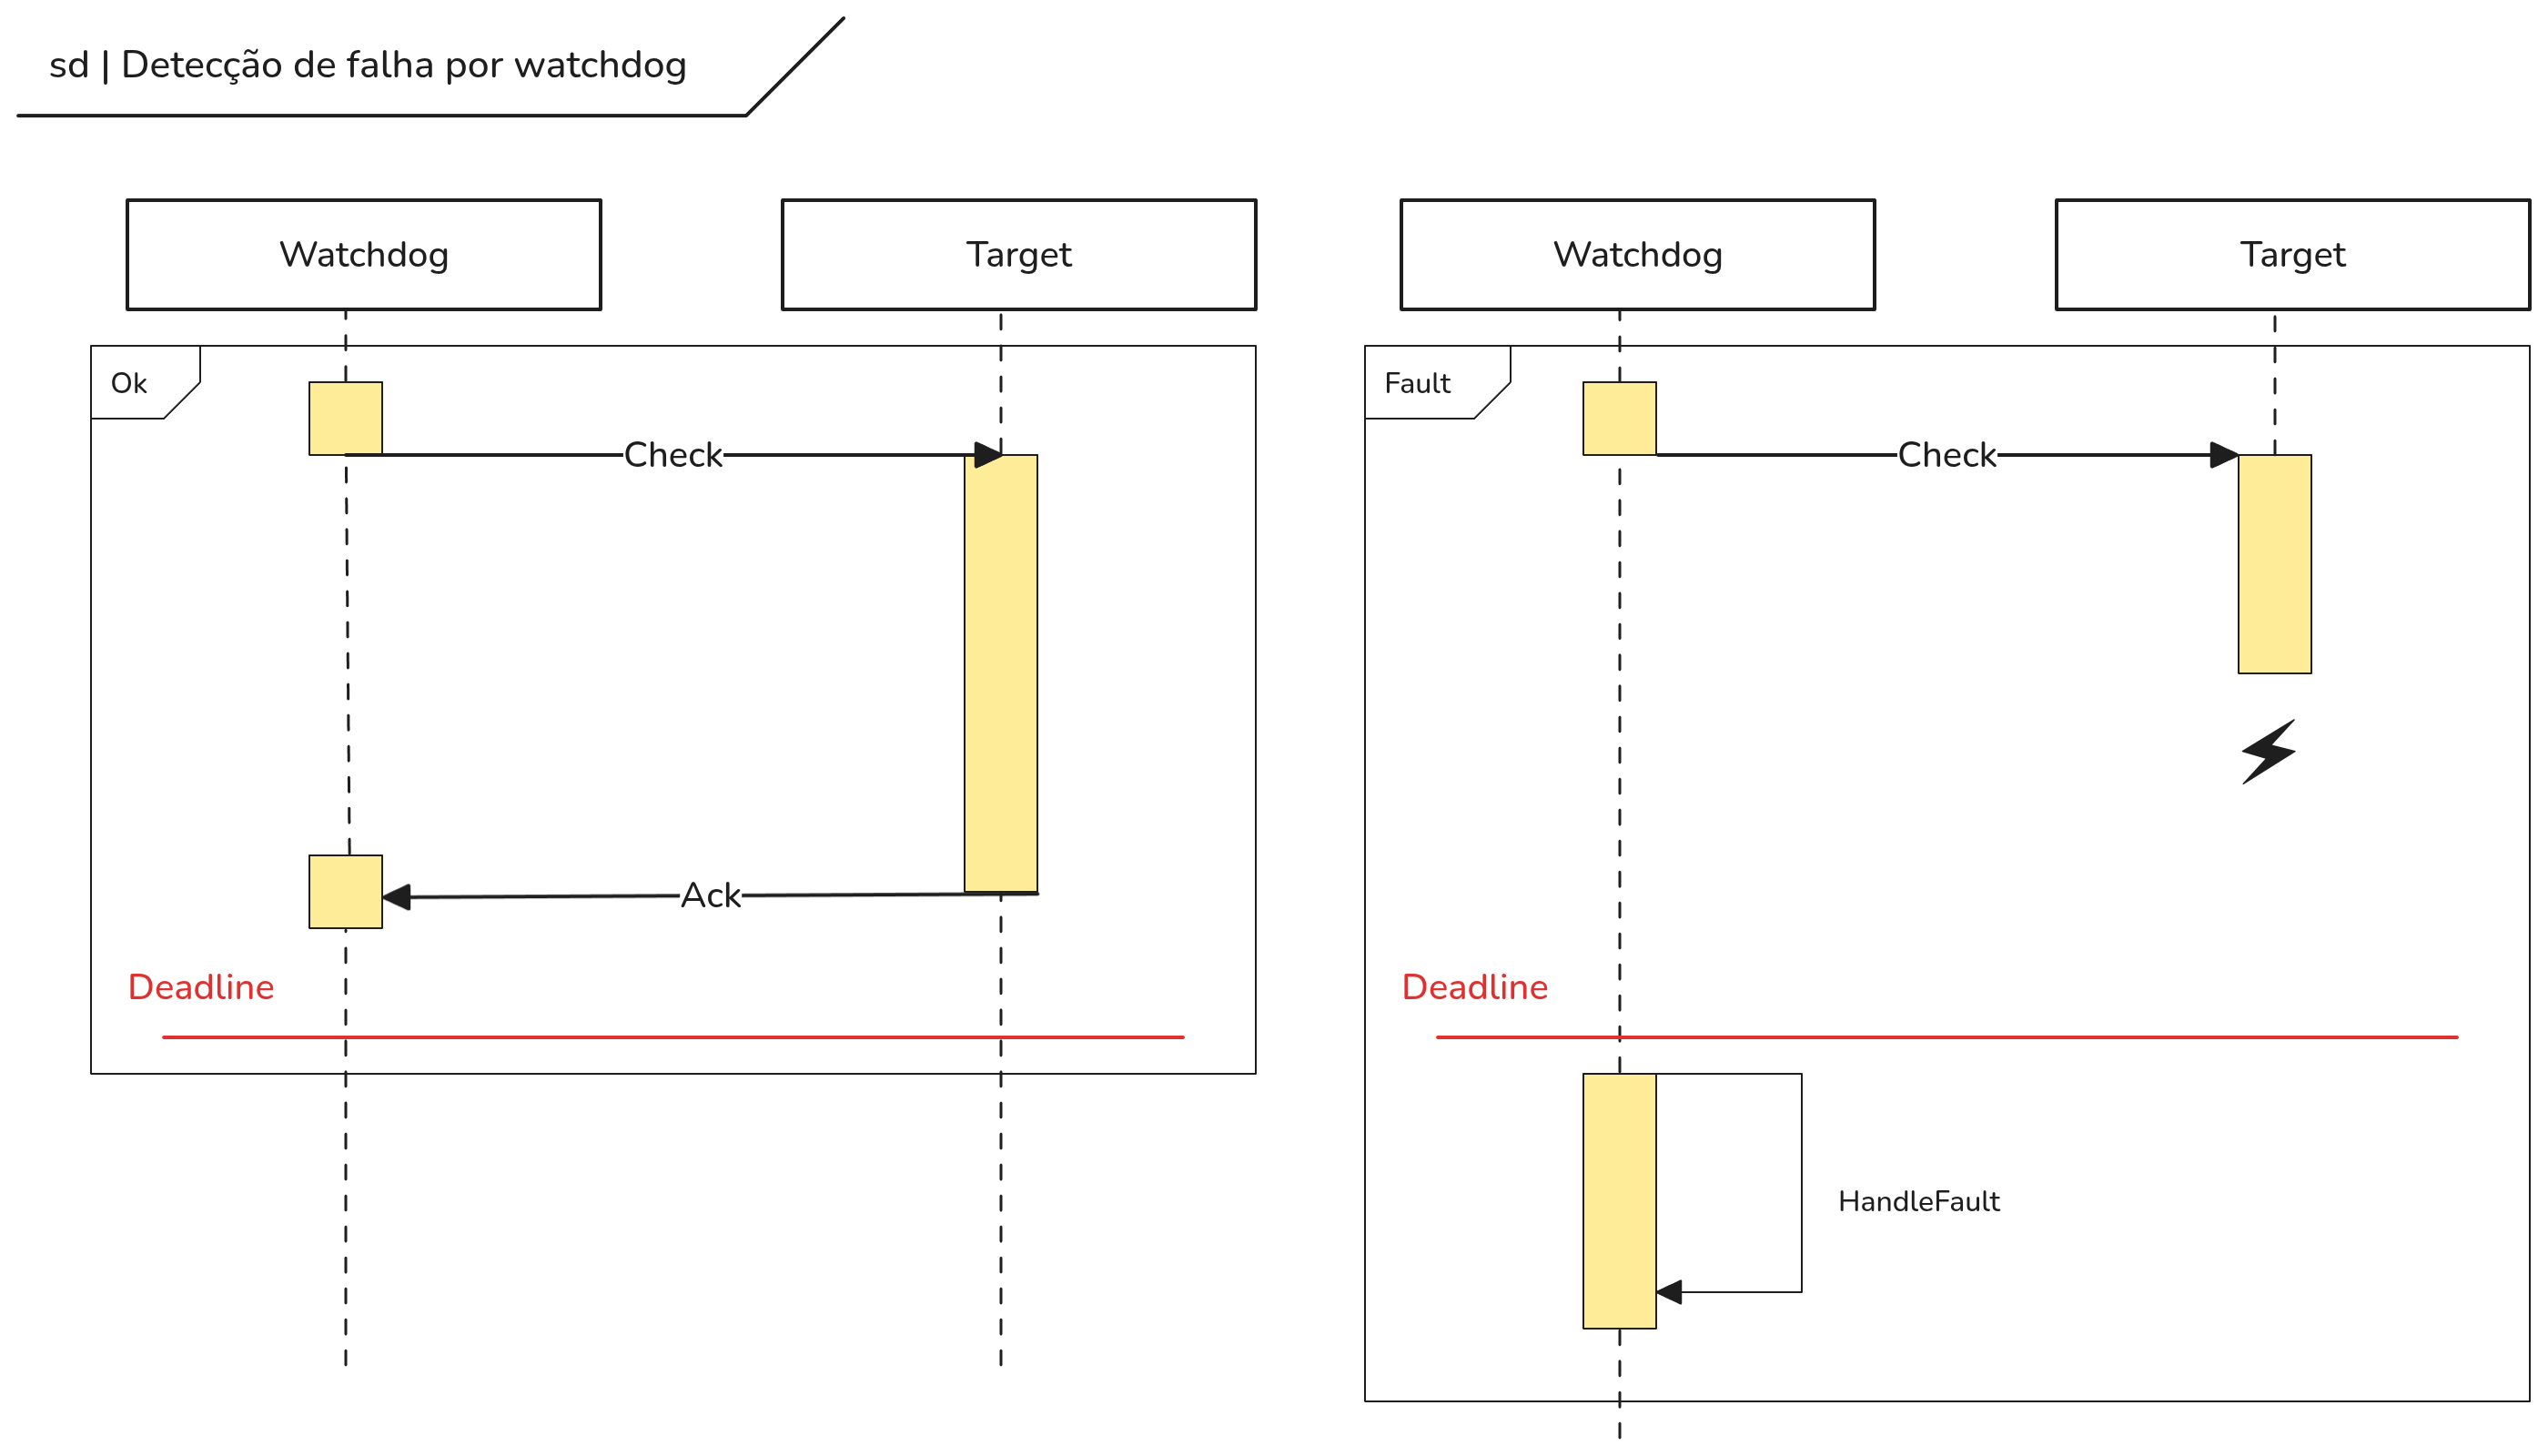
\includegraphics[width=1.0\textwidth]{assets/heartbeat_signal.png}\\
    \captionsetup{justification=raggedright}
    \caption*{Fonte: Elaborada pelo autor}
    \label{fig:heartbeatSignal}
\end{figure}

Na \autoref{fig:heartbeatSignal}, é utilizado a resposta tardia para deduzir a presença de uma falha na tarefa ou no canal de transmissão. Estes sinais também podem ser utilizados no contexto de tempo real para a validação de um prazo ou sub prazo da tarefa \cite{FaultTolerantSystems}.

\subsubsection{Asserts}

Asserts são mecanismos simples e flexíveis para a detecção de falhas, consistindo na verificação de uma condição que, durante uma execução normal do programa, deve permanecer invariavelmente verdadeira (denominada "invariante"). Caso a invariante seja falsa, detecta-se a presença de uma falha. A \autoref{fig:assert} ilustra o fluxo de um assert.

\begin{figure}[H]
    \centering
    \captionsetup{justification=centering}
    \caption{Fluxograma de um Assert}
    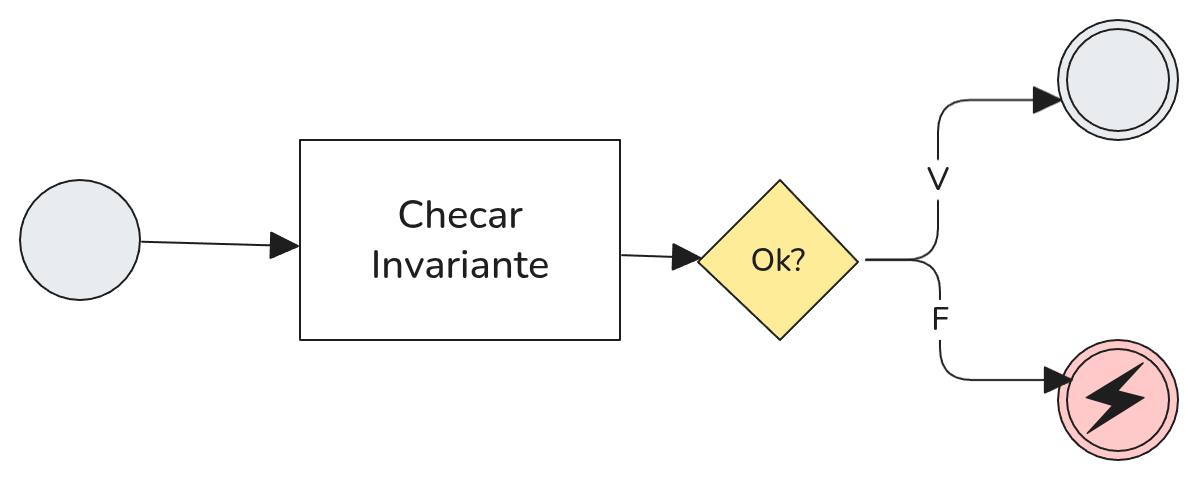
\includegraphics[width=0.5\textwidth]{assets/assert_diagram.png}\\
    \captionsetup{justification=raggedright}
    \caption*{Fonte: Elaborada pelo autor}
    \label{fig:assert}
\end{figure}

Apesar de sua simplicidade, quando usados em conjunto com simulações determinísticas e ferramentas de \textit{fuzzying}, asserts podem detectar erros durante a execução assim como revelar erros de design durante a fase de desenvolvimento \cite{TigerBeetleSafety} \cite{PowerOf10Rules}.

Durante a execução de um sistema tolerante à falhas, asserts servem como uma forma de saber rapidamente que algo errado aconteceu. Porém não são robustos o suficiente para detectar corrupção silenciosa de dados ou pulos inesperados de maneira consistente. Quando asserts são inseridos na entrada ou saída de um procedimento são denominados como pré-condições e pós-condições respectivamente. Alguns compiladores são capazes de automaticamente inserir estas condições para assegurar contratos da interface de um programa. Algumas linguagens de programação, utilizam de uma forma automática de asserts chamados de "contratos", que podem ser usados para garantir certas pós e pré condições, certos compiladores como o da linguagem SPARK fazem uso destas capacidades para realizar verificação formal de um programa \cite{SPARKContracts}.

\subsection{Mecanismos de Tratamento}

Uma vez que uma falha tenha sido detectada o sistema precisa tratar a falha o mais rápido possível para manter a qualidade de serviço, alguns mecanismos de detecção também fornecem a possibilidade de correção dos dados, como é o caso dos códigos Reed-Solomon, nestes casos, fica à critério da aplicação se a correção deve ser tentada ou outro tratamento deve ser usado.

\subsubsection{Re-execução}

Re-executar uma tarefa é uma outra forma simples de recuperar-se de uma falha, a probabilidade de $k$ falhas intermitentes ocorrem em sequência é menor do que a probabilidade de apenas ocorrer $k - 1$ vezes no intervalo de execução. Ao re-executar, espera-se que a falha não ocorra novamente na N-ésima tentativa \cite{DependabilityInEmbeddedSystems} \cite{SchedAndOptOfDistributedFT}.

Portanto, é sacrificado um tempo maior de execução caso a falha ocorra, em troca de um tempo menor de execução médio sem necessitar de componentes extras. Em contraste com a técnica de redundância tripla, é possível entender que a redundância tripla ou "tradicional", depende de uma resiliência espacial "É improvável que uma falha ocorra em vários lugares ao mesmo tempo", enquanto a re-execução depende de uma resiliência temporal: É menos provável que múltiplas falhas ocorram repetidamente em $N$ execuções \cite{FaultTolerantSystems}.

\begin{figure}[H]
    \centering
    \captionsetup{justification=centering}
    \caption{Exemplo de reexecuções}
    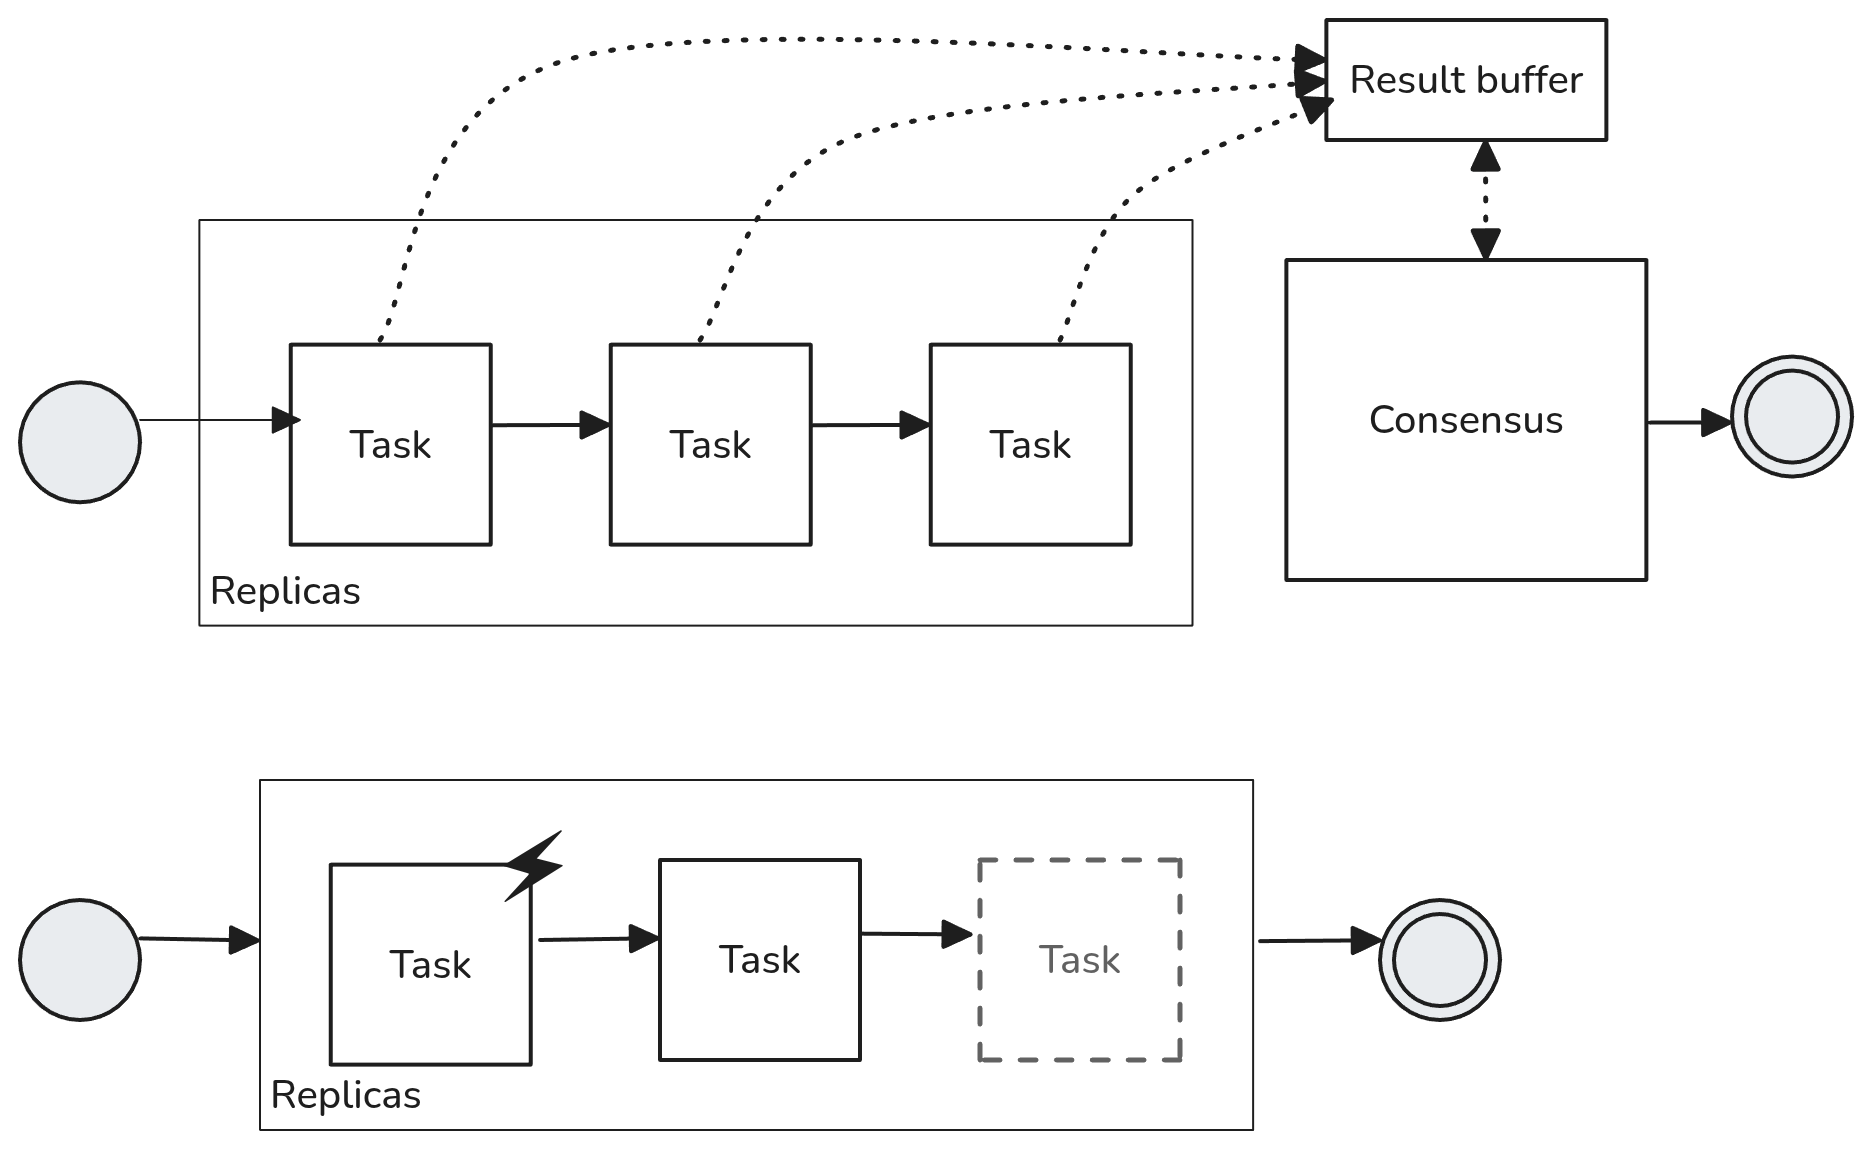
\includegraphics[width=1.0\textwidth]{assets/redundancia_reexec.png}
    \captionsetup{justification=raggedright}
    \caption*{Fonte: Elaborada pelo autor}
    \label{fig:redundanciaReexec}
\end{figure}

Na \autoref{fig:redundanciaReexec} é possível observar a reexecução de uma tarefa em duas modalidades: Na primeira é realizado um consenso entre os resultados das execuções, e na segunda a tarefa é apenas reexecutada até $N$ vezes (podendo então tolerar até $N$ falhas transientes), encerrando sua execução caso nenhuma falha seja detectada. A segunda modalidade é particularmente útil para a implementação de condições de transparência \cite{SchedAndOptOfDistributedFT} que serão abordadas posteriormente.

\subsubsection{Redundância}

Adicionar redundância ao sistema é uma das formas mais intuitivas e mais antigas de aumentar a tolerância à falhas, a probabilidade de $N$ falhas transientes ocorrendo simultaneamente em um sistema é mais baixa do que a probabilidade de apenas 1 falha \cite{SchedAndOptOfDistributedFT}.

Uma técnica de redundância comum é o uso de redundância modular, tipicamente com 3 instâncias replicadas (neste caso chamada de TMR ou "Triple Modular Redundancy"), a \autoref{fig:redundanciaTMR} ilustra a execução concorrente seguida de um votador.

O uso de TMR para uma tarefa pode consistir na reexecução concorrente das três instâncias, tendo seus resultados decidos por um votador. No contexto de tempo-real é importante que caso alguma das tasks no processo de execução concorrente viole sua deadline, que o votador ainda escolha um resultado para garantir o critério de tempo-real. O uso de TMR é elegante em sua simplicidade e consegue atingir um bom grau de resiliência, porém com o custo adicional de triplicar o custo em termos de memória e execução \cite{DependabilityInEmbeddedSystems}, e potencialmente necessitar de hardware mais poderoso para manter a mesma performance esperada.

\begin{figure}[H]
    \centering
    \captionsetup{justification=centering}
    \caption{Exemplo de execução com redundância}
    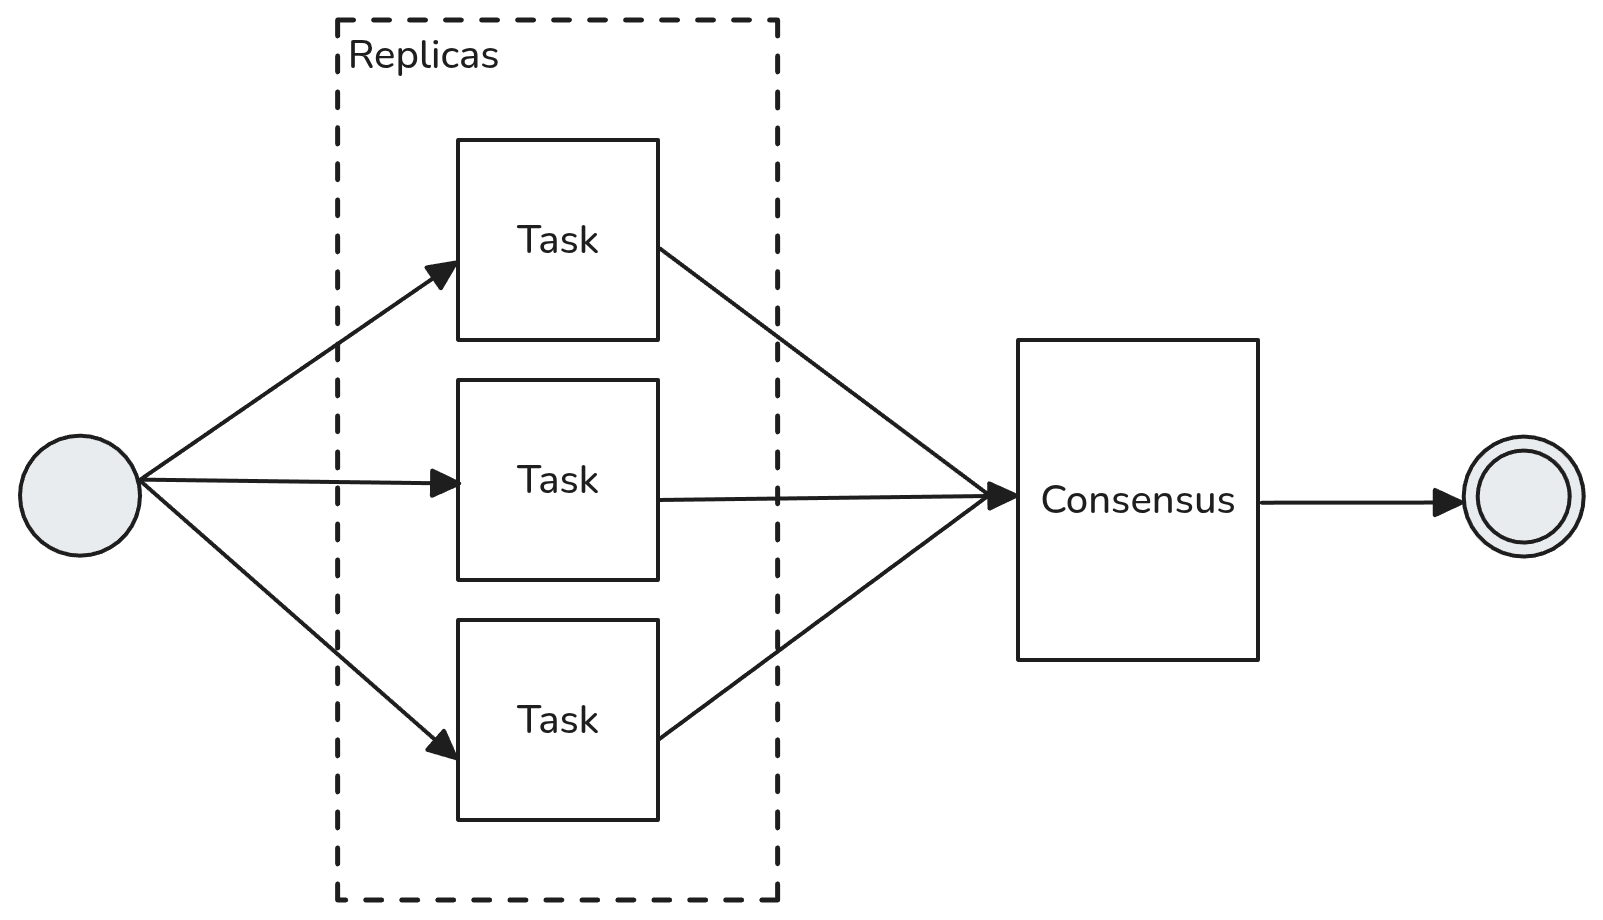
\includegraphics[width=1.0\textwidth]{assets/redundancia_tmr.png}
    \captionsetup{justification=raggedright}
    \caption*{Fonte: Elaborada pelo autor}
    \label{fig:redundanciaTMR}
\end{figure}

Sistemas distribuídos, sejam estes embarcados ou não, também podem aproveitar de sua redundância natural para ter maior dependabilidade \cite{MakingReliableDistSystems}. Falhas em um nó podem ser propagadas e no caso de falhas permanentes em um nó, os outros podem suplantar a execução de suas tarefas mantendo a qualidade média de serviço \cite{MakingReliableDistSystems} \cite{SchedAndOptOfDistributedFT}, o uso de sistemas capazes de auto reparo é vital para a existência de telecomunicação em larga escala e computação em nuvem.

\subsubsection{Loop Unrolling e Function Inlining}

Uma otimização comum que compiladores realizam é desenrolar laços de repetição (Loop Unrolling) com a finalidade de reduzir erros no preditor de desvios da CPU, no contexto de tolerância à falhas, é possível utilizar dessa otimização como uma forma de redundância espacial, ao reduzir a possibilidade de pulos dependentes de um valor, torna-se menos provável um salto baseado em uma versão corrompida do mesmo. O desenrolamento pode também ser feito caso exista um limite superior conhecido no laço durante a compilação. \cite{LoopUnrollingARM}.

Outra transformação comum é o inlining de funções, onde o corpo de uma função é copiado como se o código tivesse sido diretamente escrito em seu ponto de chamada. Ao reduzir a quantidade de pulos é possível melhorar a coerência do cache de instruções além de permitir outras otimizações durante os passes otimizantes do compilador \cite{EngineeringACompiler}, causando uma melhora na performance. No caso de tolerância à falhas, ao reduzir a quantia de jumps e prover redundância de instruções, o inlining pode também reduzir a chance de um salto inadequado \cite{MakingReliableDistSystems}. %TODO(marcos): citar aqui tbm

Importante ressaltar que aplicar \textit{function inlining} e \textit{loop unrolling} de forma excessiva pode resultar no oposto do que se deseja no quesito de performance, quando aplicadas de forma agressiva, essas otimizações saturam o cache de instruções, utilizam de mais registradores e ocupam espaço desnecessário no executável \cite{EngineeringACompiler}. Portanto, é importante que estas técnicas não sejam aplicadas de forma arbitrária e que seu uso seja acompanhado de medição para confirmar sua efetividade.

\subsection{Injeção de falhas}

Para adequadamente testar a dependabilidade do sistema, é possível deliberadamente causar falhas com o propósito de catalogar e validar se o sistema atinge as métricas necessárias. Dentre os tipos de teste que podem ser realizados, é possível categorizá-los em quatro grupos principais:

Injeção \textbf{Física}: Envolve utilizar um ambiente físico genuíno para causar as falhas, o principal benefício desta técnica é replicar eventos reais que possam causar falhas, assim como poder injetar falhas em superfícies reais do dispositivo \cite{FaultInjectionTechniques}. O principal problema é que esta técnica é particularmente cara e requer auxílio de equipamentos e profissionais especializados, também não é possível injetar um tipo específico de dado para testar um caso específico.

Injeção \textbf{Lógica em Hardware}: Utiliza-se de um dispositivo adicional para injetar as falhas que controla o dispositivo alvo, possui como vantagem ser menos intrusivo e ainda permitir um algo grau de controle e simulação dos fenômenos físicos, desvantagens incluem uma área maior de circuito necessária, implementação de uma unidade extra e criação de canais de comunicação com o dispositivo alvo \cite{FaultInjectionTechniques}.

Injeção \textbf{Lógica em Software}: Funções são executadas em software para injetar falhas em outras partes do programa, o método é pouco invasivo, de baixo custo, alta portabilidade e permite um controle muito elevado sobre os pontos de injeção e estilo de falha \cite{FaultInjectionTechniques}. Possui a desvantagem de aumentar o tempo médio de execução ao introduzir um custo extra de memória para armazenar o código de injeção, e nem sempre reproduz precisamente fenômenos físicos.

Injeção \textbf{Simulada}: O dispositivo é executado em um ambiente totalmente simulado, tem como vantagem não ser invasivo, altamente flexível e nem sequer necessitar de uma versão física do dispositivo, porém tipicamente requer software de simulação potencialmente caro assim como uma descrição do chip na forma de alguma linguagem de descrição de hardware, que raramente é disponibilizada \cite{FaultInjectionTechniques}.


\section{Sistemas embarcados}

Sistemas embarcados são uma família vasta de sistemas computacionais, algumas das principais características de sistemas embarcados são:

\textbf{Especificidade}: Diferente de um sistema de computação mais generalizado como um computador pessoal ou um servidor, sistemas embarcados são especializados para uma solução de escopo restrito. Exemplos de sistemas embarcados variam de microcontroladores encontrados em carros, televisões e dispositivos IoT até sistemas sofisticados de navegação de aeronaves e navios de grande porte \cite{ComputerOrganizationAndDesign}.

\textbf{Limitação de recursos}: Um corolário da natureza especialista destes sistemas, é que recursos alocados para o sistema são definidos previamente. No caso de microcontroladores o poder de processamento e quantidade de memória podem ser restritos para satisfazer uma necessidade de baixo custo de fabricação e menor consumo energético \cite{ComputerOrganizationAndDesign}. Importante notar que existem sistemas embarcados com acesso maior à recursos, como certos equipamentos de rede e aceleradores, mas os recursos do sistema continuam estaticamente delimitados para cumprir sua função específica.

\textbf{Critério Temporal}: Sistemas embarcados, por serem parte de um todo maior, devem realizar sua função com o mínimo de interrupção para a funcionalidade geral do contexto externo \cite{OperatingSystemConcepts}. A importância do tempo de execução de uma tarefa de um sistema pode ser classificada em duas principais categorias: Soft Real-Time , e Hard Real-Time , a distinção entre estas categorias é explicada na seção seguinte.

\subsection{Sistemas Operacionais de Tempo-Real}

Um sistema operacional é um conjunto de software que permite o gerenciamento e interação com os recursos do hardware através de uma camada de abstração. O componente essencial de um sistema operacional é o kernel, que sempre está executando, A função primordial do kernel é viabilizar a coexistência de diversas tarefas no sistema, as quais demandam acesso às capacidades do hardware, notadamente o tempo de processamento da CPU e o espaço de memória. De forma simplificada, o kernel pode ser descrito como a "cola" entre as aplicações e os recursos de hardware \cite{OperatingSystemConcepts}.

Um sistema operacional de tempo real (RTOS) é um tipo de sistema operacional mais especializado, tipicamente pequeno, que possui como característica central cumprir um critério temporal Real-Time , que é dividido em 2 categorias:

\begin{itemize}
    \item \textbf{Soft Real-Time }: Um sistema que garante essa propriedade precisa sempre garantir que tarefas de  maior importância tenham prioridade sobre as de menor importância. Sistemas Soft Real-Time  tipicamente operam na escala de milissegundos, isto é, percepção humana \cite{SchedAndOptOfDistributedFT}. O atraso de uma tarefa em um sistema Soft Real-Time  não é desejável, mas não constitui uma falha. Exemplos: Player de DVD, videogames, kiosks de atendimento automáticos.
    
    \item \textbf{Hard Real-Time }: Precisam garantir as propriedades de Soft Real-Time , além disso, o atraso de uma tarefa de seu prazo, é inaceitável, para um sistema Hard Real-Time  uma resposta com atraso é o mesmo que resposta nenhuma. Cuidado adicional deve ser utilizado ao projetar sistemas Hard Real-Time , pois muitas vezes aparacem em contextos críticos \cite{ModernOperatingSystems}. Exemplos: Software para sistema de frenagem, sistemas de navegação em aplicações aeroespaciais, software de negociação de alta frequência, fila de mensagens de alta performance
\end{itemize}

Como sistemas que cumprem o critério Hard Real-Time também cumprem os requisitos Soft Real-Time, os sistemas operacionais de tempo real tipicamente tem sua arquitetura orientada a serem capazes de cumprir o critério Hard Real-Time  \cite{SchedAndOptOfDistributedFT}.

Diferentemente de sistema operacionais focados em uso geral como Windows, Linux e OSX, os RTOSes não priorizam fornecer ao usuário uma sensação de fluidez e adaptabilidade. Devido à seus requisitos temporais rígidos, um RTOS é feito com um foco significativo em determinismo, confiabilidade e simplicidade, para garantir que tarefas sejam executadas com um respeito estrito de seus prazos \cite{OperatingSystemConcepts}. Exemplos de RTOS disponíveis no mercado incluem: FreeRTOS, VxWorks, Zephyr e LynxOS.

\subsection{Escalonador}

O escalonador é o componente do sistema operacional responsável por gerenciar múltiplas tarefas que desejam executar \cite{OperatingSystemConcepts}, sendo um componente extramente crucial, a implementação do escalonador deve garantir que tarefas de alta prioridade executem antes e que a a troca de contexto seja o mais rápido possível. O algoritmo de escalonamento é o fator central para o comportamento do escalonador, sendo categorizados em dois princpais grupos:

\begin{itemize}
    \item \textbf{Cooperativos}: Tarefas precisam voluntariamente devolver o controle da CPU (com exceção de certas interrupções de hardware) para que as outras tarefas possam executar, isso pode ser feito explicitamente por uma função de largar ou implicitamente ao utilizar uma rotina assíncrona do sistema, como ler arquivos, receber pacotes de rede ou aguardar um evento \cite{OperatingSystemConcepts}.

    \item \textbf{Preemptivos}: Além de poderem transferir a CPU manualmente, o escalonador forçará trocas de contexto caso uma condição para a troca seja satisfeita. O algoritmo mais comum que serve de base para diversos escalonadores preemptivos é o Round-Robin onde tarefas possuem uma quantia de tempo máximo alocada para sua execução contínua, nomeada "fatia de tempo" ou "quantum" \cite{ModernOperatingSystems}. Tarefas ainda podem possuir relações de prioridade, alterando a ordem que o escalonador realiza seu despache assim como o tamanho de sua fatia de tempo.
\end{itemize}

Sistemas operacionais de tempo real são tipicamente executados no modo totalmente preemptivo, mas o uso cooperativo também é viável e possui a vantagem de possuir um controle mais granular da execução das tarefas, mas é importante que seja tomado o cuidado adequado para que nenhum prazo de execução Hard Real-Time seja violado por uma tarefa inadvertidamente utilizando a CPU por uma quantidade longa de tempo.

\subsection{Concorrência e Assincronia}

Será utilizado a definição de concorrência como a habilidade de um sistema de lidar com múltiplas tarefas computacionais dividindo seus recursos (particularmente tempo de CPU e memória). Isto é, um sistema não necessariamente precisa ser paralelo (execuções múltiplas simultâneas) para possuir concorrência, mas para tornar paralelismo viável, o sistema necessita de mecanismos de concorrência \cite{MakingReliableDistSystems}.

Uma característica central para a utilidade de concorrência mesmo em situações em que paralelismo é limitado ou impossível vai além da pura expressividade do programador, existem assimetrias grandes na velocidade de acesso de disco, memória, rede, e caches da CPU como demonstrado na \autoref{fig:latencia}. Para acessar recursos de forma eficaz, é necessário lidar com suas características inerentemente assíncronas. O uso de concorrência permite que uma tarefa seja suspensa e resumida (voluntariamente ou não) o que permite que o sistema não fique excessivamente ocioso \cite{OperatingSystemConcepts}.

\begin{figure}[H]
    \centering
    \captionsetup{justification=centering}
    \caption{Hierarquia de latência de acessos}
    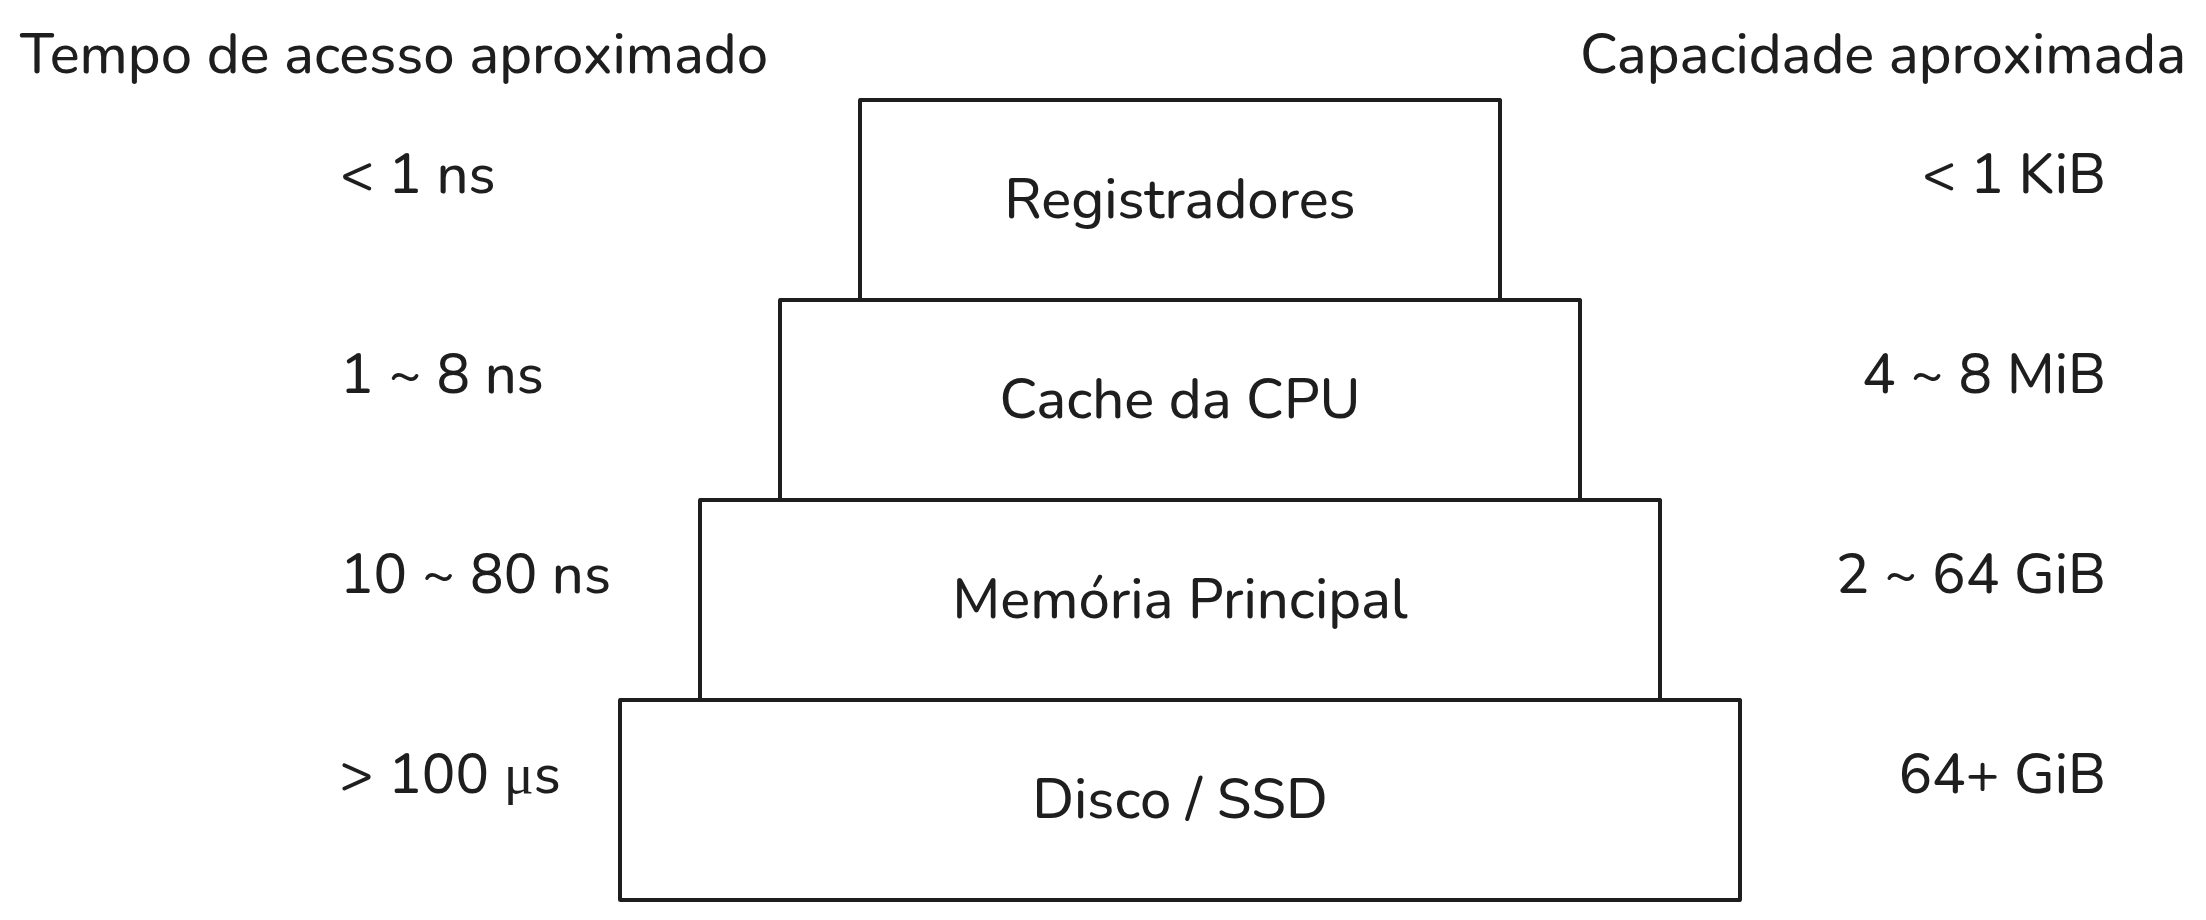
\includegraphics[width=0.8\textwidth]{assets/latency_pyramid.png}
    \captionsetup{justification=raggedright}
    \caption*{Fonte: Adaptado de \citefigure{ModernOperatingSystems}}
    \label{fig:latencia}
\end{figure}

Implementar os mecanismos de concorrência adequados também permite lidar com interrupções de forma mais estruturada, um problema clássico de lidar com uma interrupção é restaurar a memória de pilha e registradores de forma adequada, interrupções introduzem um fluxo de programa não local
%TODO livro de iface e impl em c
, violando as garantias fortes de escopo e ponto de entrada fornecidas por funções.

É uma tendência atual aumentar o número de núcleos em dispositivos, com velocidades de relógio das CPUs possuindo ganhos marginais em relação ao impacto térmico, a maioria dos computadores de propósito geral (smartphones, tablets, desktops) tipicamente possuem 2 núcleos ou mais \cite{ComputerOrganizationAndDesign}. Essa tendência não se restringe apenas à computadores gerais, sistemas embarcados comerciais também podem se beneficiar tremendamente das possibilidades de concorrência providas por mais de um núcleo, porém, é importante ressaltar que o uso de estado compartilhado se torna muito mais sensível à erros em um ambiente com múltiplos fluxos de execução, e medidas devem ser tomadas para evitar condições de corridas e deadlocks \cite{OperatingSystemConcepts}.

\subsection{Execução de Tarefas na Presença de Falhas}

Para uma representação mais clara e eficaz de um fluxo de execução sujeito a falhas, é possível utilizar de grafos resilientes a falhas como um mecanismo de diagramação. Nesta representação, os nós correspondem a tarefas, as quais podem ser executadas na mesma unidade de processamento ou não. As arestas do grafo representam o fluxo de execução, uma aresta não demarcada indica execução incondicional, enquanto arestas demarcadas com notação de mensagem designam uma execução condicional à transmissão de uma mensagem. Mensagens e tarefas representadas por símbolo circular indicam pontos ordinários no grafo, ao passo que símbolos quadrados denotam condições de transparência. \cite{SchedAndOptOfDistributedFT}.

Um grafo de processos tolerantes é falhas é definido como um grafo não ponderado direcionado acíclico com seus nós representando tarefas/processos, arestas representam o fluxo de execução e arestas nomeadas representam fluxo dependente da entrega de mensagens. Será utilizado a notação $P_X (N)$, onde $X$ é o número identificador da tarefa, e $N$ corresponde à sua $N$-ésima re-execução, por exemplo: $P_2 (1)$ indica a primeira execução da tarefa $P_2$, enquanto $P_1 (3)$ indica a terceira reexecução da tarefa $P_1$. Uma notação similar será utilizada para mensagens entre tarefas, $m_X (N)$, mensagens, assim como tarefas, estão sujeitas à falhas e custos adicionais de detecção, mas ao invés de re-execução, mensagens são re-enviadas \cite{SchedFTWithSoftAndHardConstraints}.

Para melhor exemplificar a importância da detecção das falhas, será tomado como exemplo um grafo simples, com apenas 3 tarefas e uma mensagem. O grafo precisará tolerar uma falha transiente. O fluxo "ideal" é demonstrado na \autoref{fig:ftgSimples}.

\begin{figure}[H]
    \centering
    \captionsetup{justification=centering}
    \caption{Grafo com 3 processos e uma mensagem}
    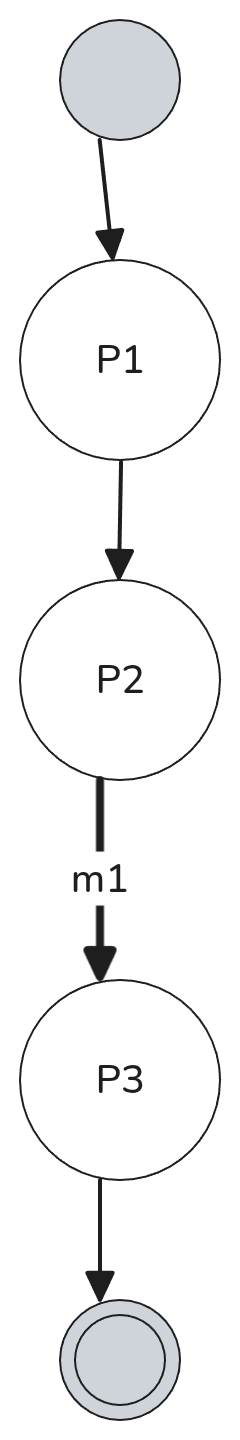
\includegraphics[width=0.120\textwidth]{assets/ftg_simples.png}
    \captionsetup{justification=raggedright}
    \caption*{Fonte: Elaborada pelo autor}
    \label{fig:ftgSimples}
\end{figure}

Ao incluir os diferentes desvios possíveis na presença de apenas uma falha, o grafo de execução da \autoref{fig:ftgExpandido} é obtido. A incidência de falhas no processamento ou passagem de mensagens é indicada com um ícone de raio.

\begin{figure}[H]
    \centering
    \captionsetup{justification=centering}
    \caption{Mesmo grafo, mas tolerante à uma falha transiente}
    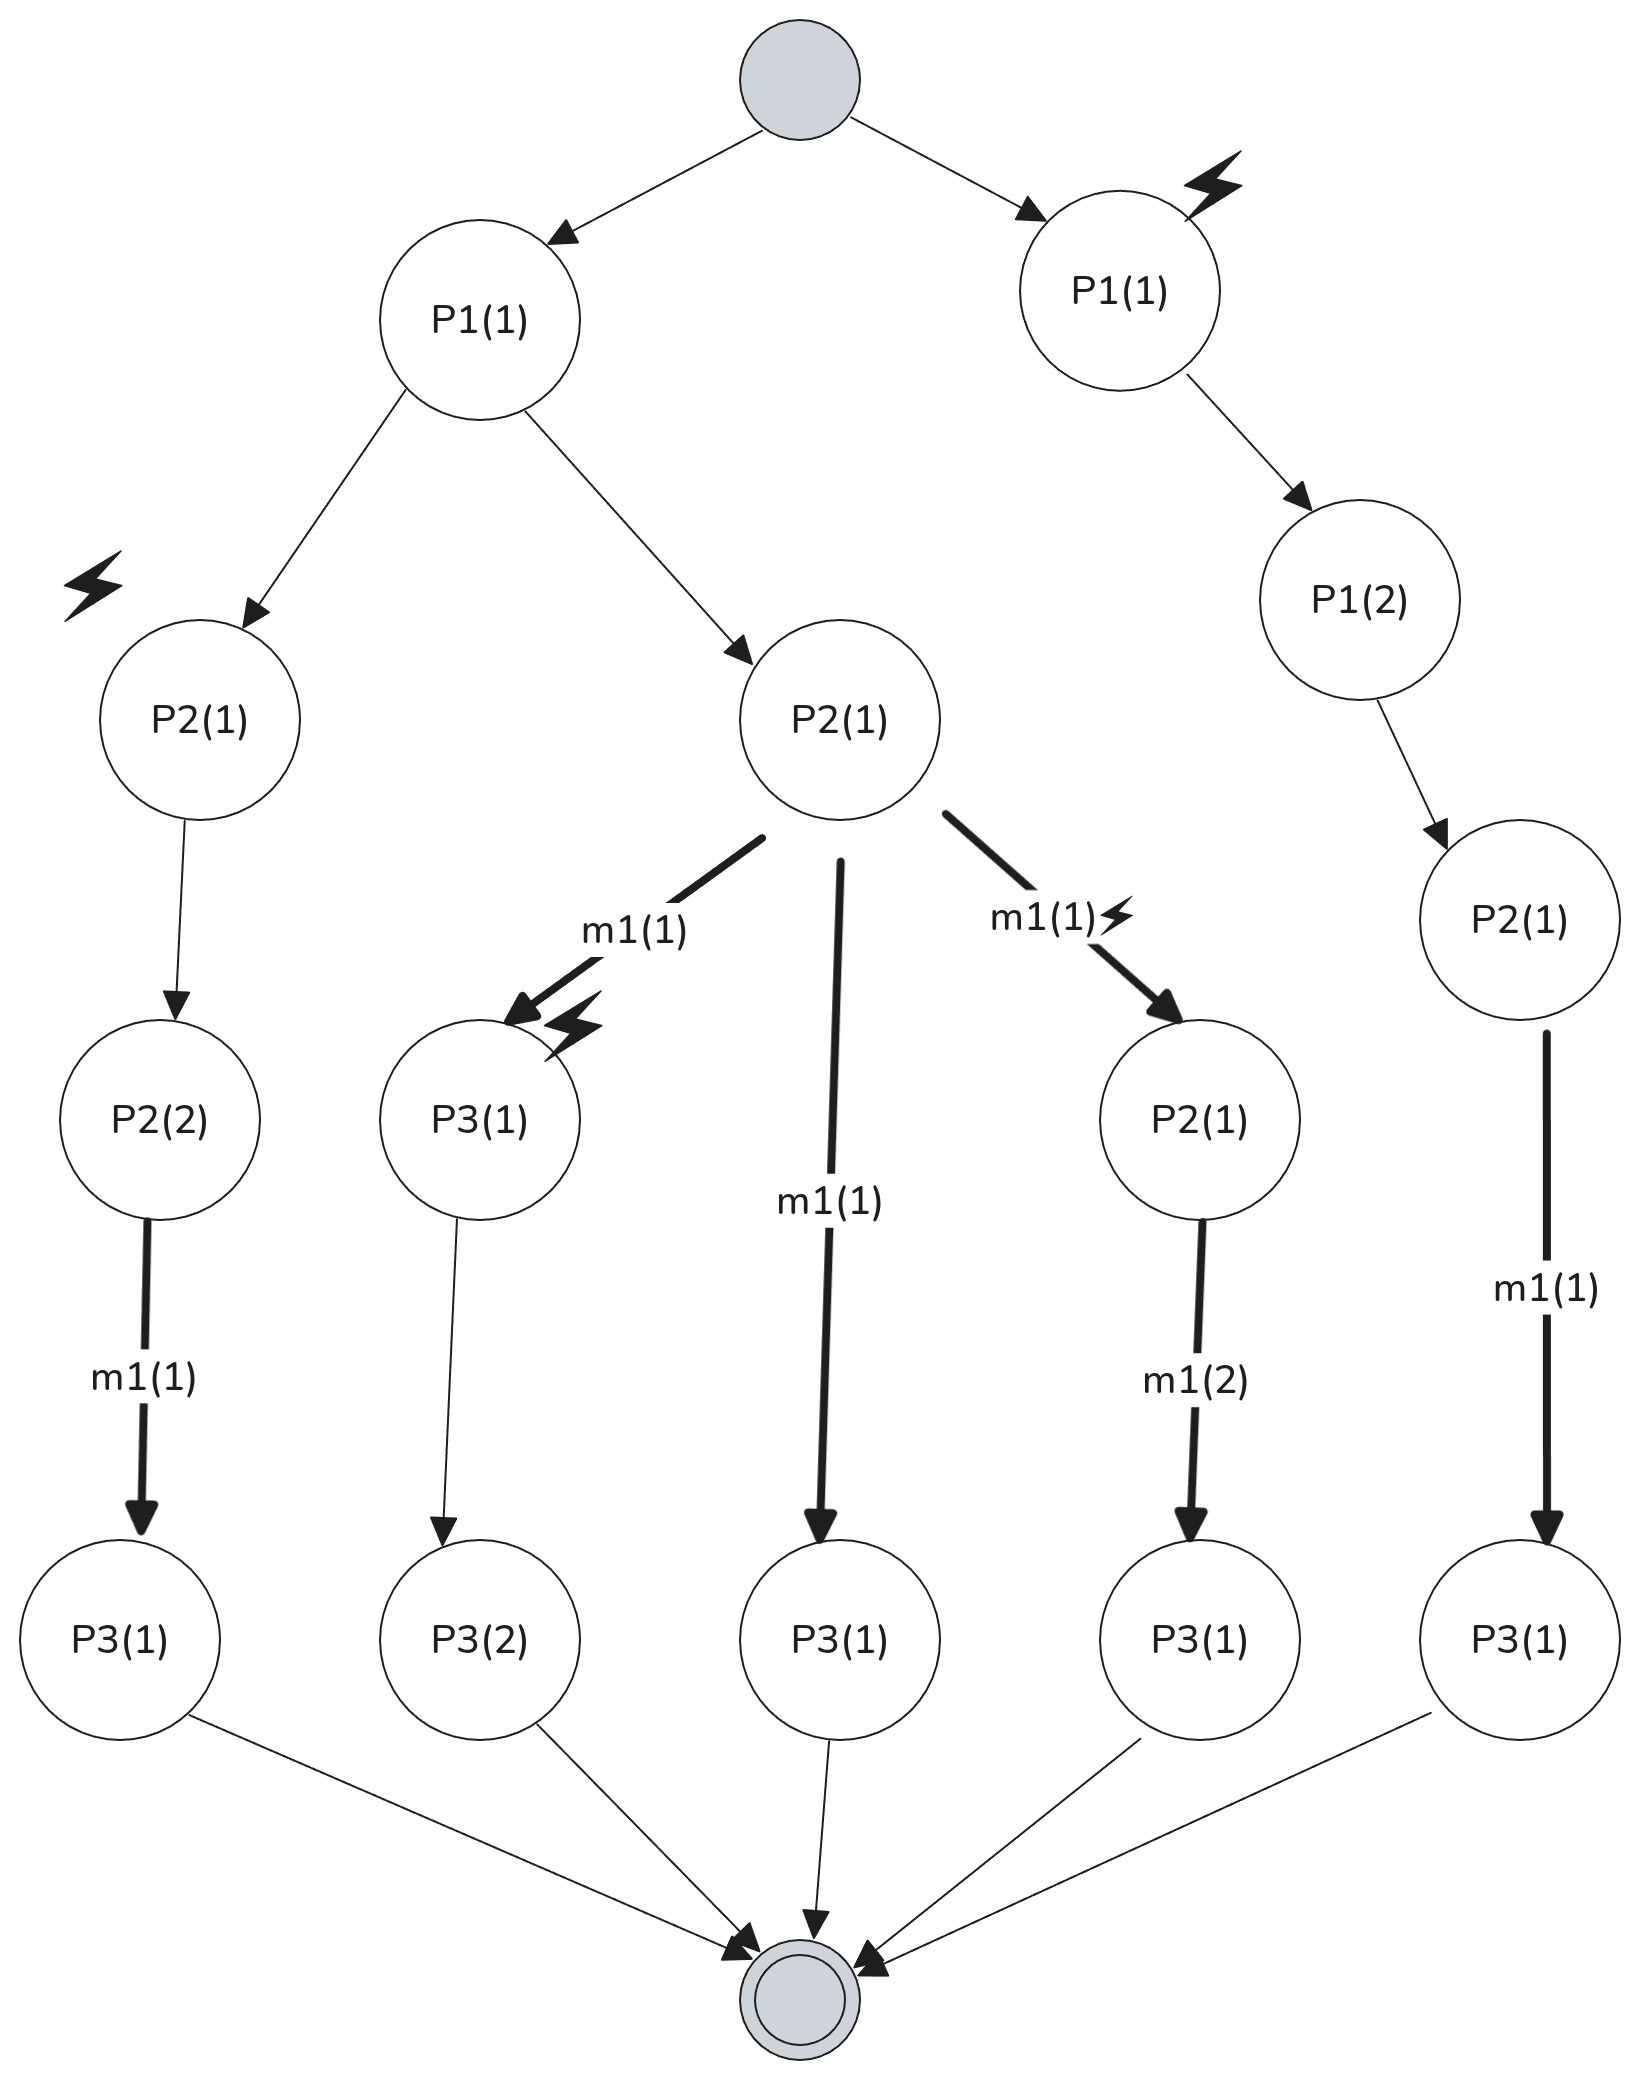
\includegraphics[width=0.75\textwidth]{assets/ftg_expandido.png}
    \captionsetup{justification=raggedright}
    \caption*{Fonte: Elaborada pelo autor}
    \label{fig:ftgExpandido}
\end{figure}

Será introduzido transparência na tarefa $P_2$, isto é, será executada com redundância temporal ou modular de tal forma que as tarefas subsequentes pudessem assumir "como se" uma falha nunca tivesse acontecido em $P_2$ após sua deadline ter sido completa, o grafo na \autoref{fig:ftgTransparencia} demonstra a condição de transparência com um ícone retangular.

\begin{figure}[H]
    \centering
    \captionsetup{justification=centering}
    \caption{Introdução de transparência em $P_2$}
    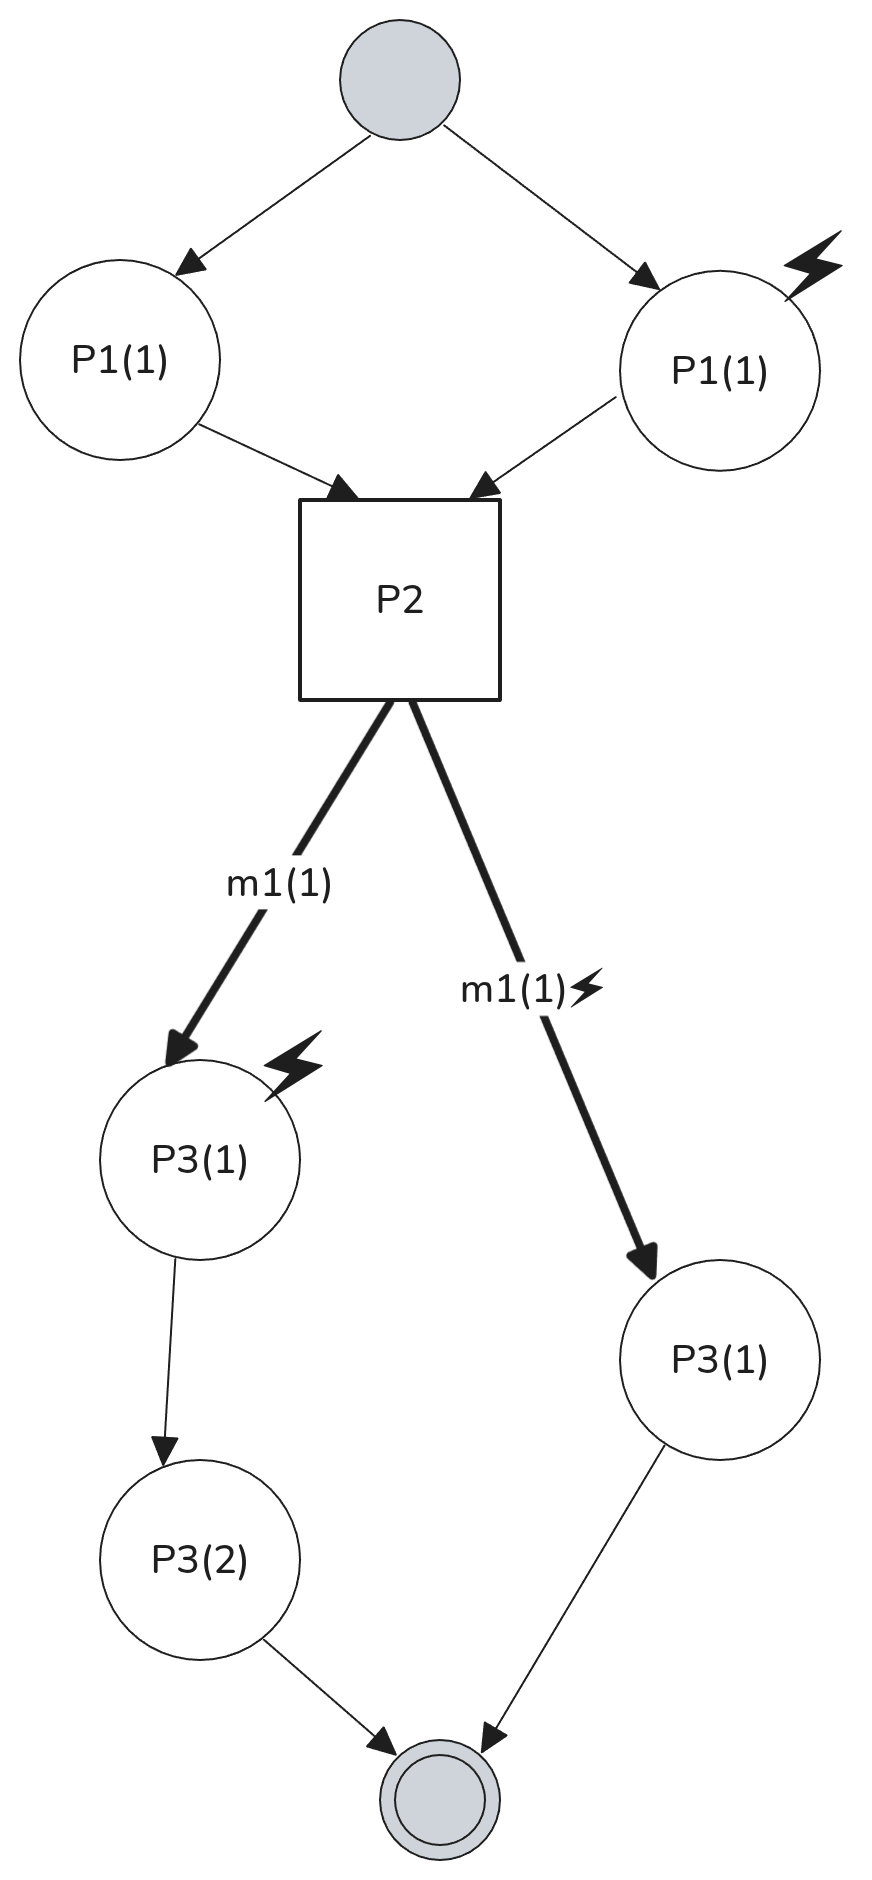
\includegraphics[width=0.40\textwidth]{assets/ftg_transparencia.png}
    \captionsetup{justification=raggedright}
    \caption*{Fonte: Elaborada pelo autor}
    \label{fig:ftgTransparencia}
\end{figure}

Introduzindo apenas um ponto de transparência é possível reduzir significativamente as possibilidades de execução do sistema, isso é particularmente benéfico para escalonadores ou algoritmos de tratamento de falhas baseados em máquinas de estado finito. Um grafo mais compacto é benéfico a previsibilidade do sistema, estabelecendo uma relação forte de pré-conclusão com sucesso ao respeitar o prazo da tarefa transparente \cite{SchedAndOptOfDistributedFT}.

Este exemplo é simples e tolera apenas uma falha transiente, porém processos complexos com múltiplas mensagens entre si causam um aumento exponencial de complexidade, especialmente caso seja necessário tolerar até $k$ falhas transientes.

Pode-se adicionar pontos de transparência através de reexecução ou redundância modular (se a deadline conjunta das $N$ tarefas for determinística) para aumentar a confiabilidade e previsibilidade do sistema. Essa transparência não é gratuita: há um troca entre maior confiabilidade no escalonador e menor imprevisibilidade na execução, com o custo de maior uso de CPU e memória. Todos os pontos precisam ser verificados, o que pode aumentar o tempo ocioso dos núcleos e exigir a extensão do prazo da tarefa para permitir reexecuções suficientes.

\section{Trabalhos relacionados} \label{sec:trabRel}

Durante a pesquisa bibliográfica para a fundamentação deste trabalho, foram selecionados três artigos que abordassem temas de tolerância à falhas em software.

\subsection{Reliability Assessment of Arm Cortex-M Processors under Heavy Ions and Emulated Fault Injection}

No trabalho de \citeindirect{ReliabilityArmCortexUnderHeavyIons} utilizam de um sistema COTS e criam um perfil de falhas com exposição a íons pesados assim como injeção artificial de falhas em software para posteriormente realizar uma adição de formas de detecção de falhas para melhorar a confiabilidade do sistema. Foi possível detectar mais da metade das falhas funcionais apenas com técnicas de software, como indicado na figura \autoref{fig:trabRelIonsPesados}.

\begin{figure}[H]
    \centering
    \captionsetup{justification=centering}
    \caption{Análise de resiliência, dividida por categoria}
    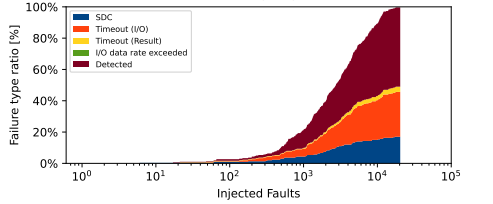
\includegraphics[width=0.75\textwidth]{assets/related_works_heavy_ion_reliability.png}
    \captionsetup{justification=raggedright}
    \caption*{Fonte: \citefigure{ReliabilityArmCortexUnderHeavyIons}}
    \label{fig:trabRelIonsPesados}
\end{figure}

Uma outra observação foi que a memória foi duas ordens de magnitude maior em relação ao banco de registradores, indicando que é necessário um foco maior na detecção de falhas na memória \cite{ReliabilityArmCortexUnderHeavyIons}.

\subsection{Técnica de confiabilidade em nível de sistema operacional para a arquitetura RISC-V}

O trabalho de \citeindirect{TecnicaConfiabilidadeRISCV} aborda uma aplicação de TMR (Replicação com $N = 3$) dos processos em um microkernel para a arquitetura RISC-V, para a validação da implementação é utilizado injeção de falhas lógicas em software emuladas com o depurador GDB e o com QEMU como emulador, o sistema é escrito na linguagem Rust que é capaz de fornecer garantias de segurança de acessos à memória. Foi observado um aumento de confiabilidade do sistema em troca de um custo adicional de memória e tempo de execução.

\subsection{Application-Level Fault Tolerance in Real-Time Embedded System}

No trabalho de \citeindirect{ApplicationLevelFT} são apresentada técnicas de tolerância à falhas em um sistema operacional chamado BOSS, é utilizado uma interface de thread com a implementação de tolerância conformando à interface. O trabalho naturalmente explora o escalonador mas não entra em detalhamento profundo na parte de detecção, mas sim de prover uma biblioteca na forma de classes representando tarefas resilientes \cite{ApplicationLevelFT}. Um caso de estudo de um sistema de filtragem de radar é utilizado como projeto.

O trabalho demonstra também a viabilidade de prover interfaces mais abstratas que ainda sejam capazes de executar em sistemas de recursos restritos. Demonstraram-se resultados favoráveis para uma forma híbrida de tolerância com menor uso de CPU em relação à redundância tripla utilizando de técnicas em software combinado com um par de processadores com auto checagem (PSP).

\subsection{Análise Comparativa dos trabalhos relacionados}

Após comparar os trabalhos, o de natureza mais similar em termos de arquitetura é o de \citeindirect{ApplicationLevelFT} e o mais similar em termos de técnicas de injeção e materiais utilizados a técnica de confiabilidade apresentada em \citeindirect{TecnicaConfiabilidadeRISCV}. O \autoref{tab:trabRel} demonstra as principais diferenças entre os trabalhos.

\begin{quadro}[H]
    \centering
    \caption{Comparação dos trabalhos relacionados}
    \begin{tabular}{|p{0.20\textwidth}|p{0.15\textwidth}|p{0.15\textwidth}|p{0.15\textwidth}|p{0.20\textwidth}|}
        \hline
        \rowcolor[HTML]{C0C0C0}
        \textbf{Trabalho} & \textbf{Sistema} & \textbf{Hardware} & \textbf{Injeção} & \textbf{Técnicas} \\
        \hline

        \citefigure{ReliabilityArmCortexUnderHeavyIons} & Bare Metal, FreeRTOS & CY8CKIT-059 & Física e Lógica em Software & Redundância de Registradores, Deadlines, Redução de Registradores, Asserts \\
        \hline

        \citefigure{TecnicaConfiabilidadeRISCV} & RISC-V Emulado no QEMU & Microkernel de \citeindirect{BasicMicrokernelForRISCV} & Emulada em Software & Redundância Modular, Segurança de memória extra (Borrow checker do Rust) \\
        \hline

        \citefigure{ApplicationLevelFT} & BOSS & Máquinas PowerPC 823 e um PC x86\_64 não especificado & Simulada em Software & Redundância Modular, Deadlines, Rollback/Retry \\
        \hline

        Este Trabalho & FreeRTOS & STM32 Bluepill & Lógica em Software e Hardware & Deadlines, Heartbeat, Asserts, Reexecução e Redundância de Tarefas \\
        \hline

    \end{tabular}
    \label{tab:trabRel}
\end{quadro}

 \clearpage
\chapter{Projeto}
\label{cap:proj}

\section{Visão Geral}

Serão implementados mecanismos de tolerância utilizando do FreeRTOS como base, as técnicas implementadas serão discutidas em maior detalhe na \autoref{subsec:algoritmos}. Para a coleta das métricas de eficácia e custo computacional será utilizado um cenário de injeção de falhas lógicas em hardware utilizando do depurador em chip ST-Link, os detalhes da campanha de injeção de falhas são abordados na \autoref{subsec:campanhaInjecao}.

A \autoref{fig:visaoGeral} sumariza a relação entre os principais componentes, as técnicas de tolerância são implementadas como complementos ao FreeRTOS e o processo de injeção é controlado por um computador externo que envia comandos para o depurador em chip com o propósito de simular uma falha.

\begin{figure}[H]
    \centering
    \captionsetup{justification=centering}
    \caption{Principais componentes do projeto}
    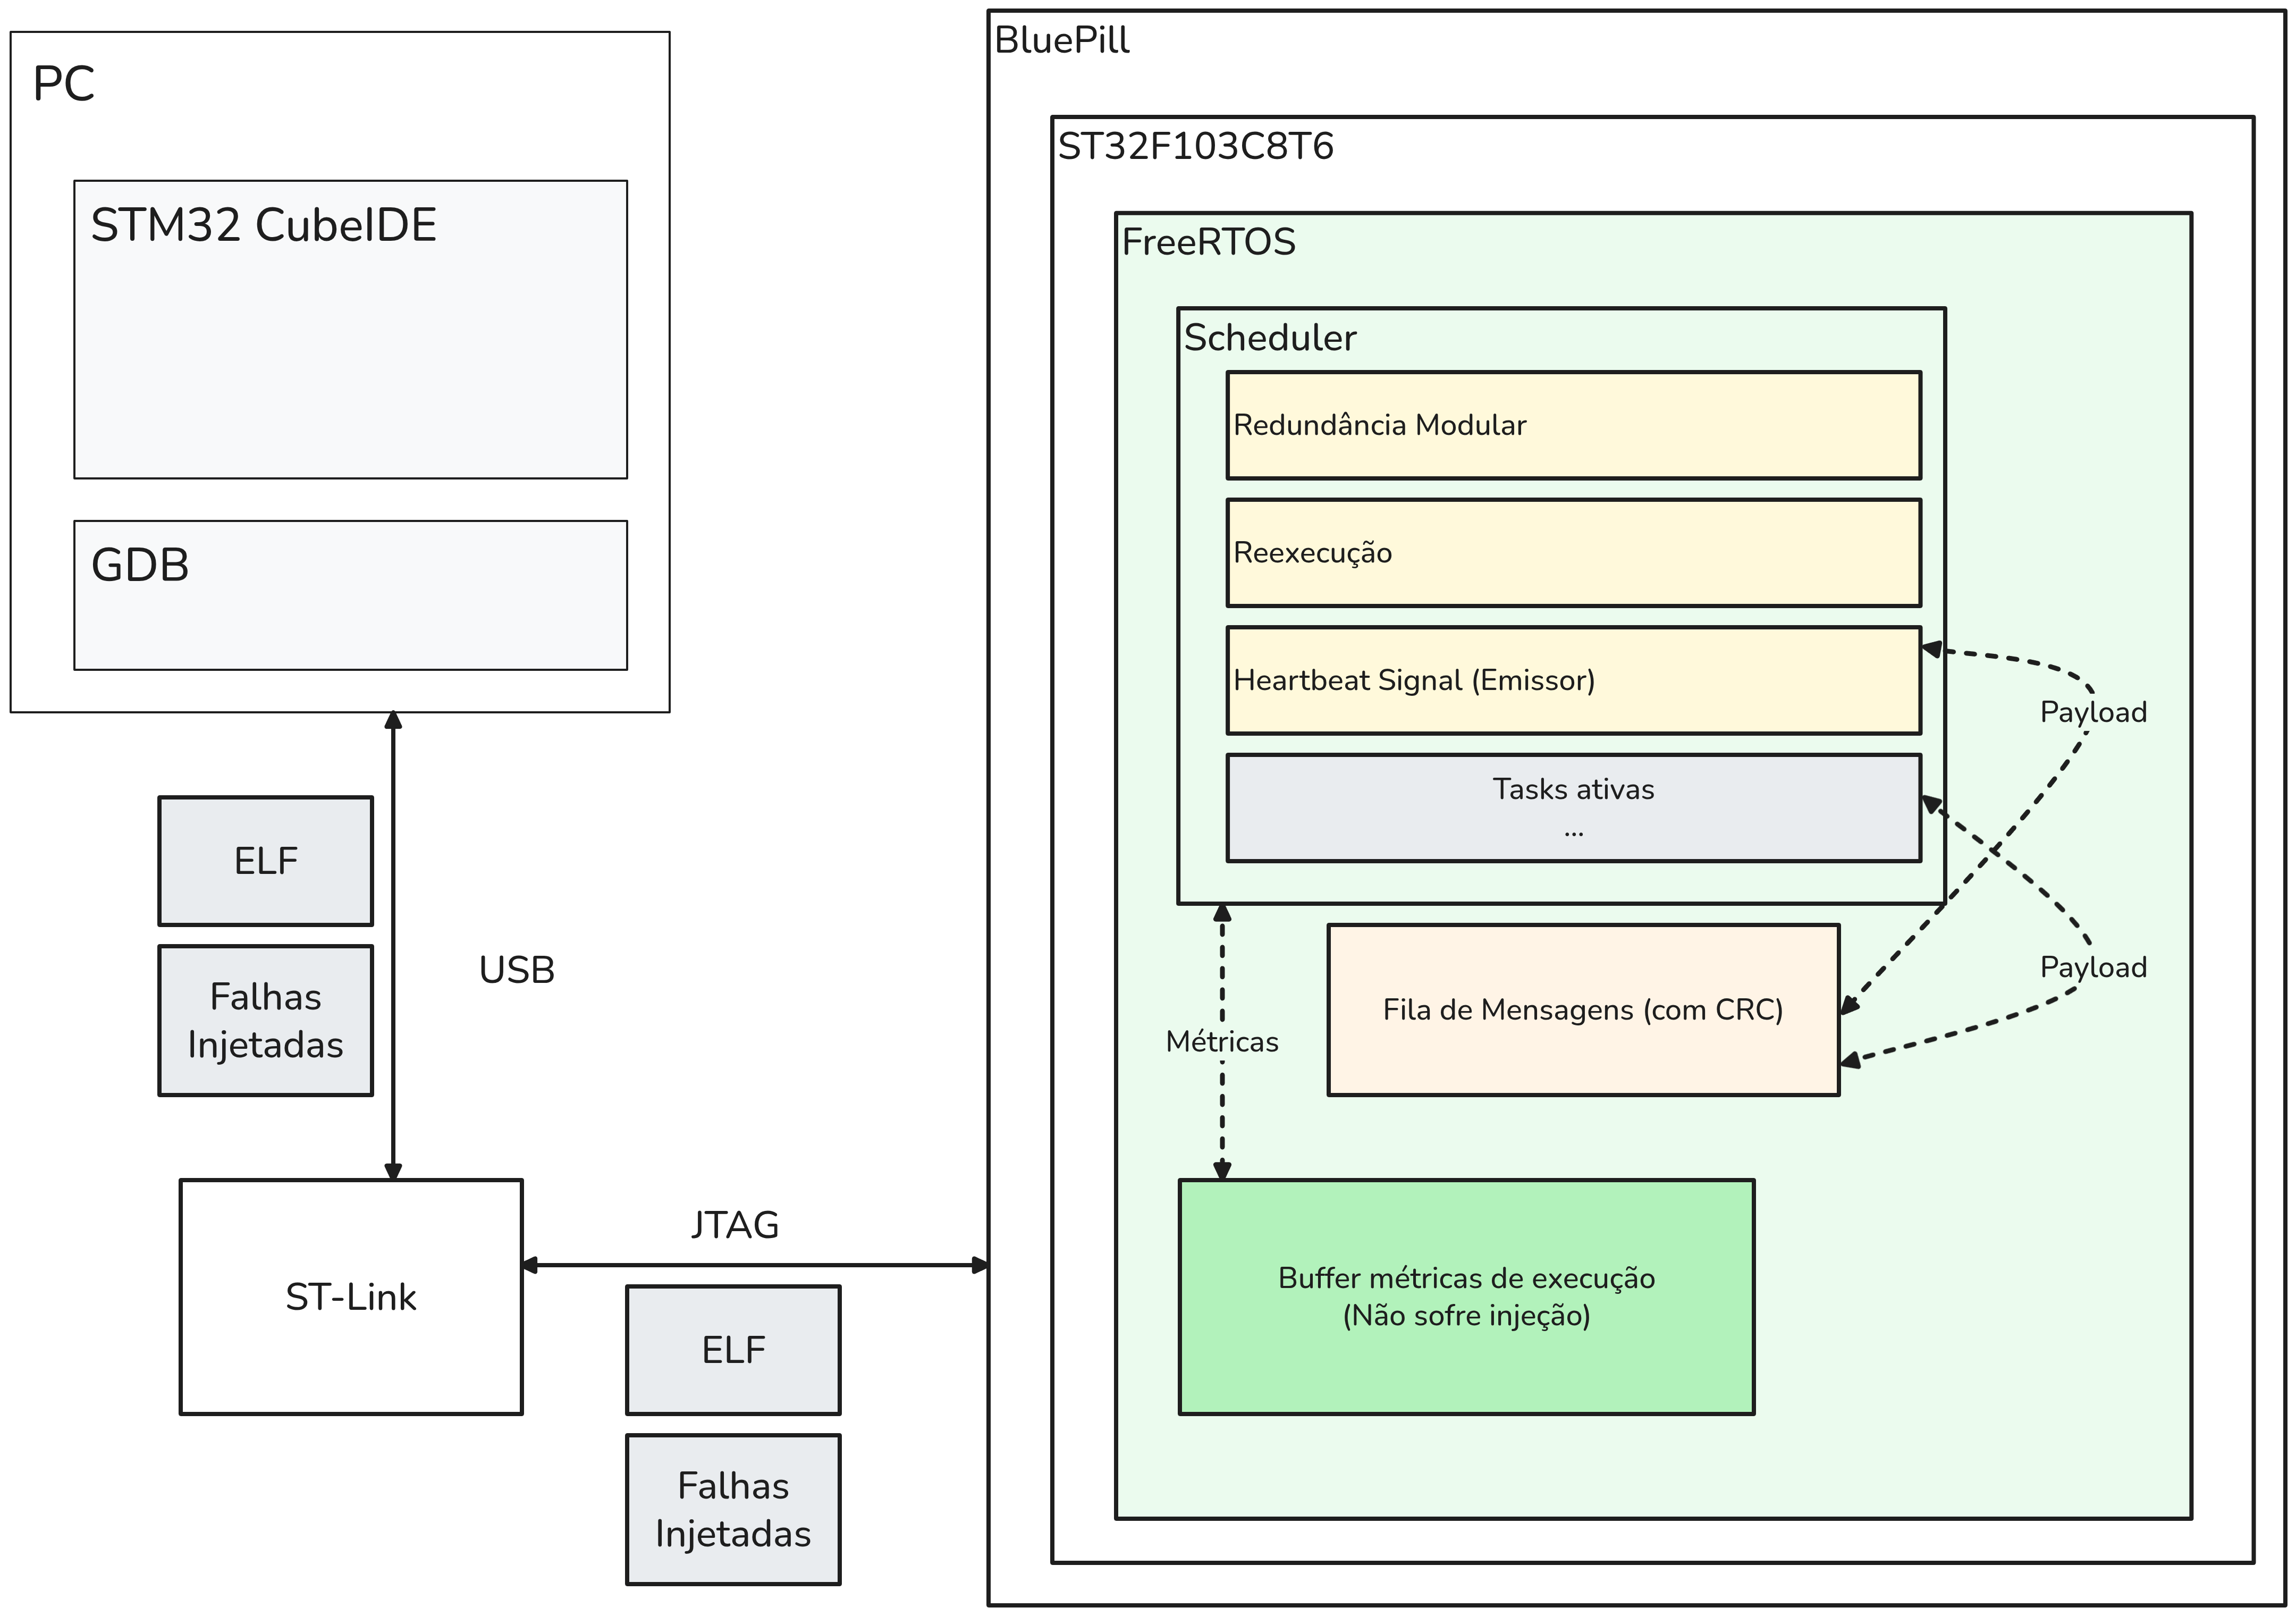
\includegraphics[width=0.97\textwidth]{assets/visao_geral.png}
    \captionsetup{justification=raggedright}
    \caption*{Fonte: Elaborada pelo autor}
    \label{fig:visaoGeral}
\end{figure}

\section{Premissas}

Será partido do ponto que ao menos o processador que executa o escalonador terá registradores de controle (ponteiro de pilha, contador de programa, endereço de retorno) que sejam capazes de mascarar falhas. Apesar de ser possível executar os algoritmos reforçados com análise de fluxo do programa e adicionar redundância aos registradores, isso adiciona um grau a mais de complexidade que foge do escopo do trabalho. Como mencionado na \autoref{sec:trabRel}, a memória fora do banco de registradores pode ser duas ordens de magnitude mais sensível à eventos disruptivos \cite{ReliabilityArmCortexUnderHeavyIons}.

O sistema tentará atingir um critério de Hard Real-Time, isto é, o descumprimento de um prazo de execução será considerado uma falha completa. Prazos de execução podem ser locais à um segmento particular do programa ou globais que correspondem ao programa como um todo ou à um macro processo. A escolha do critério Hard Real-Time também é útil de um ponto de vista da análise pois será possível comparar o custo temporal da aplicação de técnicas em relação ao limite de execução.

Com o fim de reduzir o tamanho do executável e manter o fluxo de mais previsível não serão utilizados mecanismos de exceção com desenrolamento (\textit{unwinding}) da pilha. Também não será utilizado de RTTI (Runtime Type Information). Todos os erros devem portanto ser tratados como valores ou como falhas lógicas.

Necessariamente, é preciso também presumir que testes sintéticos possam ao menos aproximar a performance do mundo real, ou ao menos prever o pior caso possível com grau razoável de acurácia. O uso de testes sintéticos não deve ser um substituto para a medição em uma aplicação real, porém, uma bateria de testes com injeção artificial de falhas pode ser utilizada para verificar as tendências e custos relativos introduzidos, mesmo que não necessariamente reflitam as medidas absolutas do produto final.

Portanto, será assumido que os resultados extraídos de injeção de falhas artificiais, apesar de menos condizentes com os valores absolutos de uma aplicação e não sendo substitutos adequados na fase de aprovação de um produto real, são ao menos capazes para realizar uma análise quanto ao custo proporcional introduzido, e devido à sua facilidade de realização e profundidade de inspeção possível, serão priorizados inicialmente neste projeto.

\section{Metodologia}

\subsection{Materiais}

Será utilizada a linguagem C++ com o compilador GCC (ou Clang), o alvo principal do trabalho será um microcontrolador STM32F103C8T6 "Bluepill" 32-bits da arquitetura ARMv7-M, como visto na \autoref{fig:stm32Bluepill}.

\begin{figure}[H]
    \centering
    \captionsetup{justification=centering}
    \caption{Diagrama da STM32F103C8T6 ("Bluepill")}
    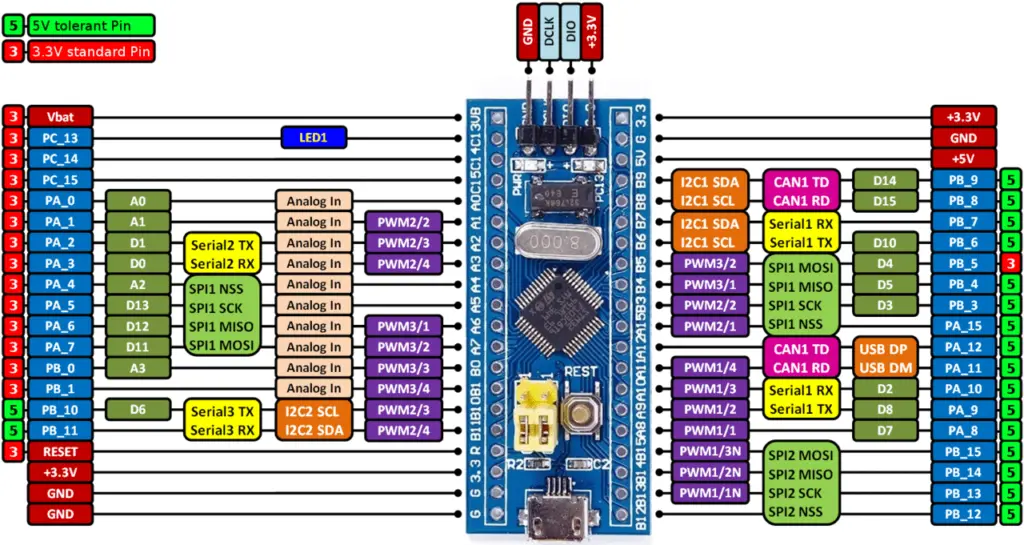
\includegraphics[width=0.80\textwidth]{assets/stm32_bluepill.png}
    \captionsetup{justification=raggedright}
    \caption*{Fonte: \citefigure{STMBoardProductPage}}
    \label{fig:stm32Bluepill}
\end{figure}

Para a injeção de falhas será utilizado o depurador GDB em conjunto com uma ferramenta de depuração de hardware ST-LINK (\autoref{fig:stLink}), a comunicação do ST-LINK é feita via USB com o computador e via JTAG com o microcontrolador alvo, também será usado em conjunto uma IDE fornecida pelo mesmo fabricante, a STM32Cube IDE.

\begin{figure}[H]
    \centering
    \captionsetup{justification=centering}
    \caption{ST-LINK/V2}
    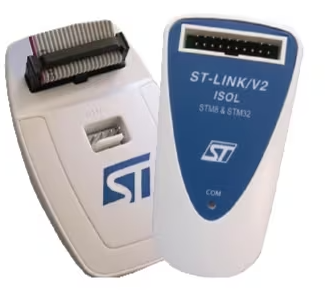
\includegraphics[width=0.40\textwidth]{assets/st_link.png}
    \captionsetup{justification=raggedright}
    \caption*{Fonte: \citefigure{STLinkProductPage}}
    \label{fig:stLink}
\end{figure}

\begin{figure}[H]
    \centering
    \captionsetup{justification=centering}
    \caption{STMCubeIDE}
    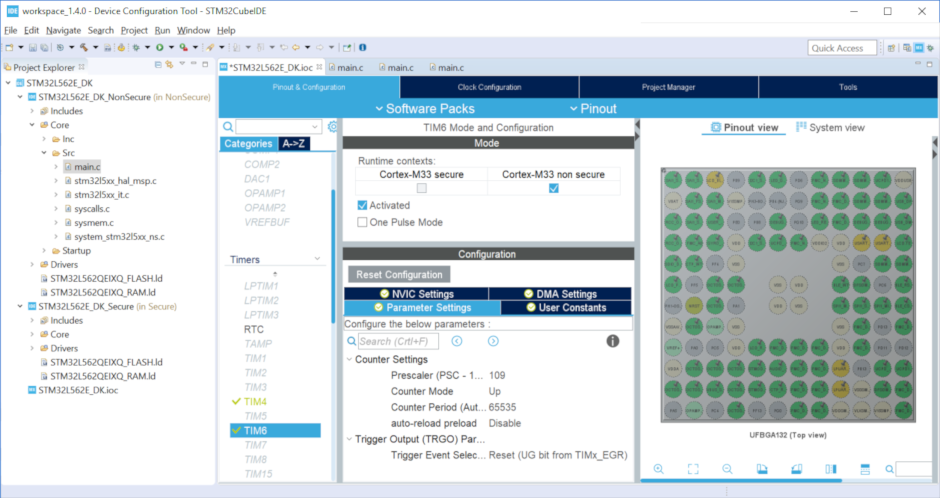
\includegraphics[width=0.65\textwidth]{assets/stmcube_ide.png}
    \captionsetup{justification=raggedright}
    \caption*{Fonte: \citefigure{STMCubeProductPage}}
    \label{fig:stmCubeIDE}
\end{figure}

Durante a fase de desenvolvimento dos algoritmos será utilizado o QEMU juntamente com as ferramentas anteriormente citadas, assim como sanitizadores de memória e condições de corrida (ASan, TSan, UBSan) para auxiliar na detecção de erros mais cedo durante o desenvolvimento.

O sistema operacional de tempo real escolhido foi o FreeRTOS, por ser extensivamente testado e documentado e prover um escalonador totalmente preemptivo com um custo espacial relativamente pequeno, além disso, os contribuidores do FreeRTOS mantém uma lista grande de versões para diferentes arquiteturas e controladores, facilitando drasticamente o trabalho ao não ter que criar uma HAL do zero.

\subsection{Métodos}

Serão utilizadas as seguintes técnicas de tolerância à falhas implementadas em software: CRCs para mensagens, redundância modular, reexecução, sinal heartbeat e asserts. O detalhamento específico de cada técnica é abordado em maior detalhe na \autoref{subsec:algoritmos}.

Para a criação da análise, serão realizados testes com injeção lógica em hardware utilizando-se do ST-Link em combinação com um computador que emitirá os comandos para injeção via depurador, as falhas serão de natureza transiente e afetarão valores na memória (corrupção silenciosa) assim como nos registradores que não são de controle. A \autoref{fig:injecaoHardwareLogica} detalha de forma mais específica o fluxo de gerar uma falha. As combinações específicas de falhas e técnicas escolhidas são abordadas na \autoref{subsec:campanhaInjecao}.

\begin{figure}[H]
   \centering
   \captionsetup{justification=centering}
   \caption{Injeção lógica em hardware}
   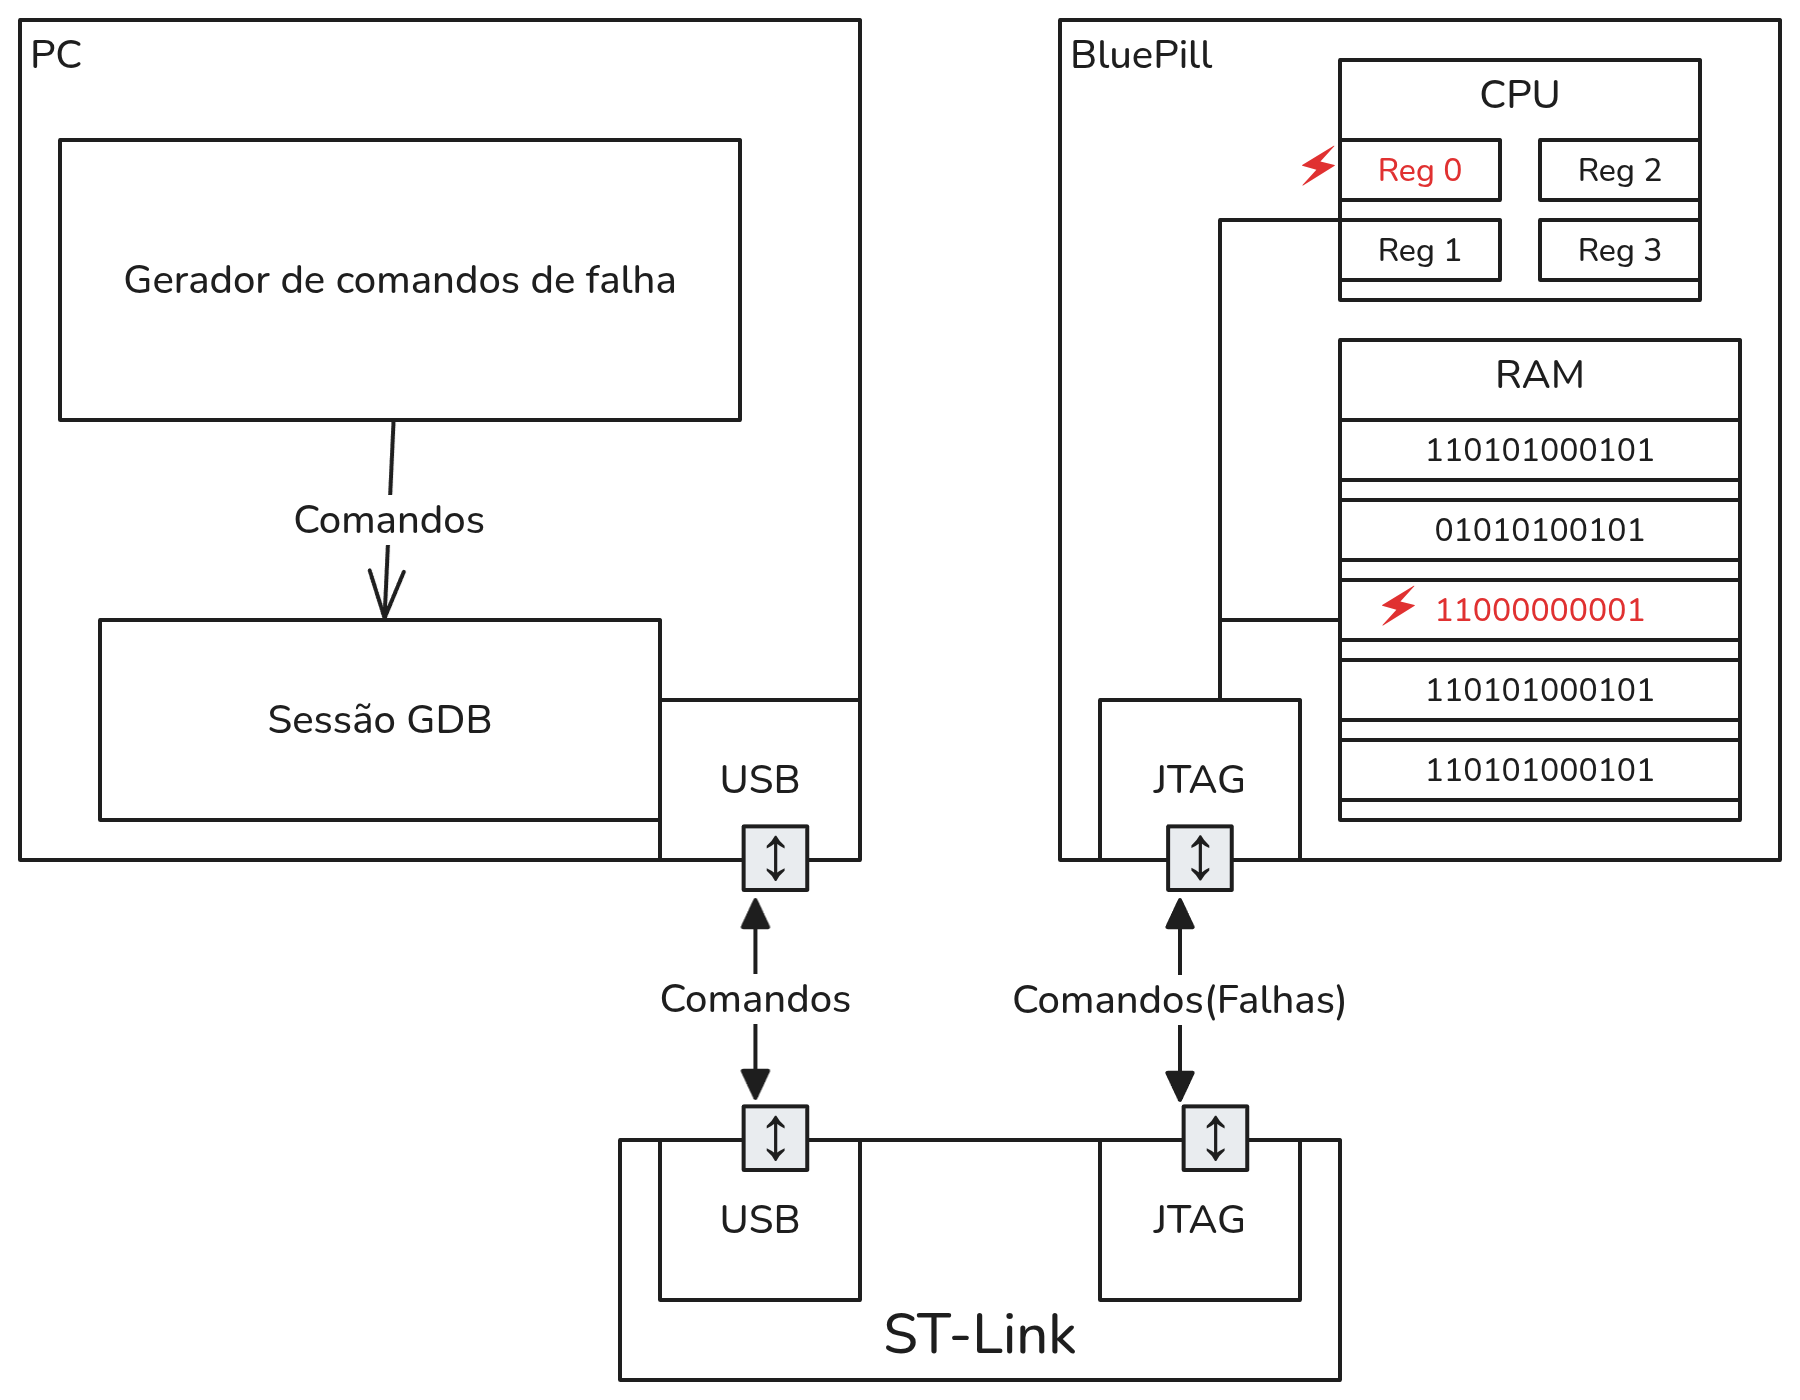
\includegraphics[width=0.85\textwidth]{assets/injecao_hardware.png}
   \captionsetup{justification=raggedright}
  \caption*{Fonte: Elaborada pelo autor}
   \label{fig:injecaoHardwareLogica}
\end{figure}

A coleta de métricas será realizada com os mecanismos de monitoramento do sistema FreeRTOS juntamente com contadores de incremento atômico, o tempo de execução das tarefas, seu espaço de memória utilizado e o número de falhas detectadas será armazenado em uma estrutura que residirá em um segmento de memória que é deliberadamente isento de falhas.

Com o objetivo de promover a reutilização de código e a abstração, será implementada uma interface que generaliza um objeto de tarefa. Considerando que um objeto que realiza despache dinâmico requer uma tabela de despacho virtual (V-Table), faz-se necessário adotar precauções adicionais, dado que a própria tabela pode estar sujeita a falhas. Para mitigar esse risco, será aplicada uma replicação simples dos ponteiros de função da V-Table, resultando em um custo adicional de duas comparações por chamada de método. A interação da interface com o resto do sistema é abordada em maior detalhe na \autoref{subsec:interface}.

\section{Análise de requisitos}
\label{sec:req}

\begin{quadro}[H]
    \centering
    \caption{Requisitos funcionais}
    \begin{tabular}{|p{0.125\textwidth}|p{0.8\textwidth}|}
        \hline
        \rowcolor[HTML]{C0C0C0}
        \textbf{Requisito} & \textbf{Descrição}  \\
        \hline
        
        \textbf{RF01} & Implementação de todos os algoritmos descritos na \autoref{subsec:algoritmos} \\ 
        \hline

        \textbf{RF02} & Criação, finalização e cancelamento de tarefas e recuperação de sua memória alocada \\
        \hline
        
        \textbf{RF03} & Configuração do mecanismo de tolerância, prioridade e prazo de execução da tarefa \\
        \hline

        \textbf{RF04} & Cumprimento do prazo estipulado no momento de criação da tarefa caso não exista presença de falhas \\
        \hline

        \textbf{RF05} & Dependabilidade superior à versão do sistema sem técnicas \\
        \hline
        
        \textbf{RF06} & Monitoramento do número de falhas detectadas e violações de prazos  \\
        \hline
        
        \textbf{RF07} & Comunicação entre tarefas por uma fila com checagem dos pacotes \\
        \hline
    \end{tabular}
    \label{tab:rf}
\end{quadro}

\begin{quadro}[H]
    \centering
    \caption{Requisitos não funcionais}
    \begin{tabular}{|p{0.125\textwidth}|p{0.8\textwidth}|}
        \hline
        \rowcolor[HTML]{C0C0C0}
        \textbf{Requisito} & \textbf{Descrição}  \\
        \hline
        
        \textbf{RNF01} & O consumo de memória deve ser pré determinado em tempo de compilação ou na inicialização do sistema \\
        \hline
        
        \textbf{RNF02} & A interface deve ser construida sobre o escalonador preemptivo do FreeRTOS \\
        \hline

        \textbf{RNF03} & Deve ser compatível com arquitetura ARMv7M ou ARMv8M \\
        \hline

        \textbf{RNF04} & Implementação realizada em C++ (versão 20 ou acima) \\
        \hline
        
        \textbf{RNF05} & Código fonte da interface disponível sob licença permissiva (BSD3) \\
        \hline
    \end{tabular}
    \label{tab:rnf}
\end{quadro}

\subsection{Interface} \label{subsec:interface}

Para melhor generalizar o uso das técnicas, utiliza-se de uma abstração da estrutura de tarefa juntamente com um mecanismo de passagem de mensagens com detecção de erros.

Uma mensagem envelopa um pacote de dados qualquer para que possa ser enviado de forma assíncrona entre tarefas. Neste caso, o ordenamento dos campos é importante: o pacote precisa ser o último membro para serialização de estruturas de tamanho arbitrário, a distribuição dos campos na memória é demonstrada na \autoref{fig:messageStruct}. 

\begin{figure}[H]
    \centering
    \captionsetup{justification=centering}
    \caption{Layout de uma mensagem}
    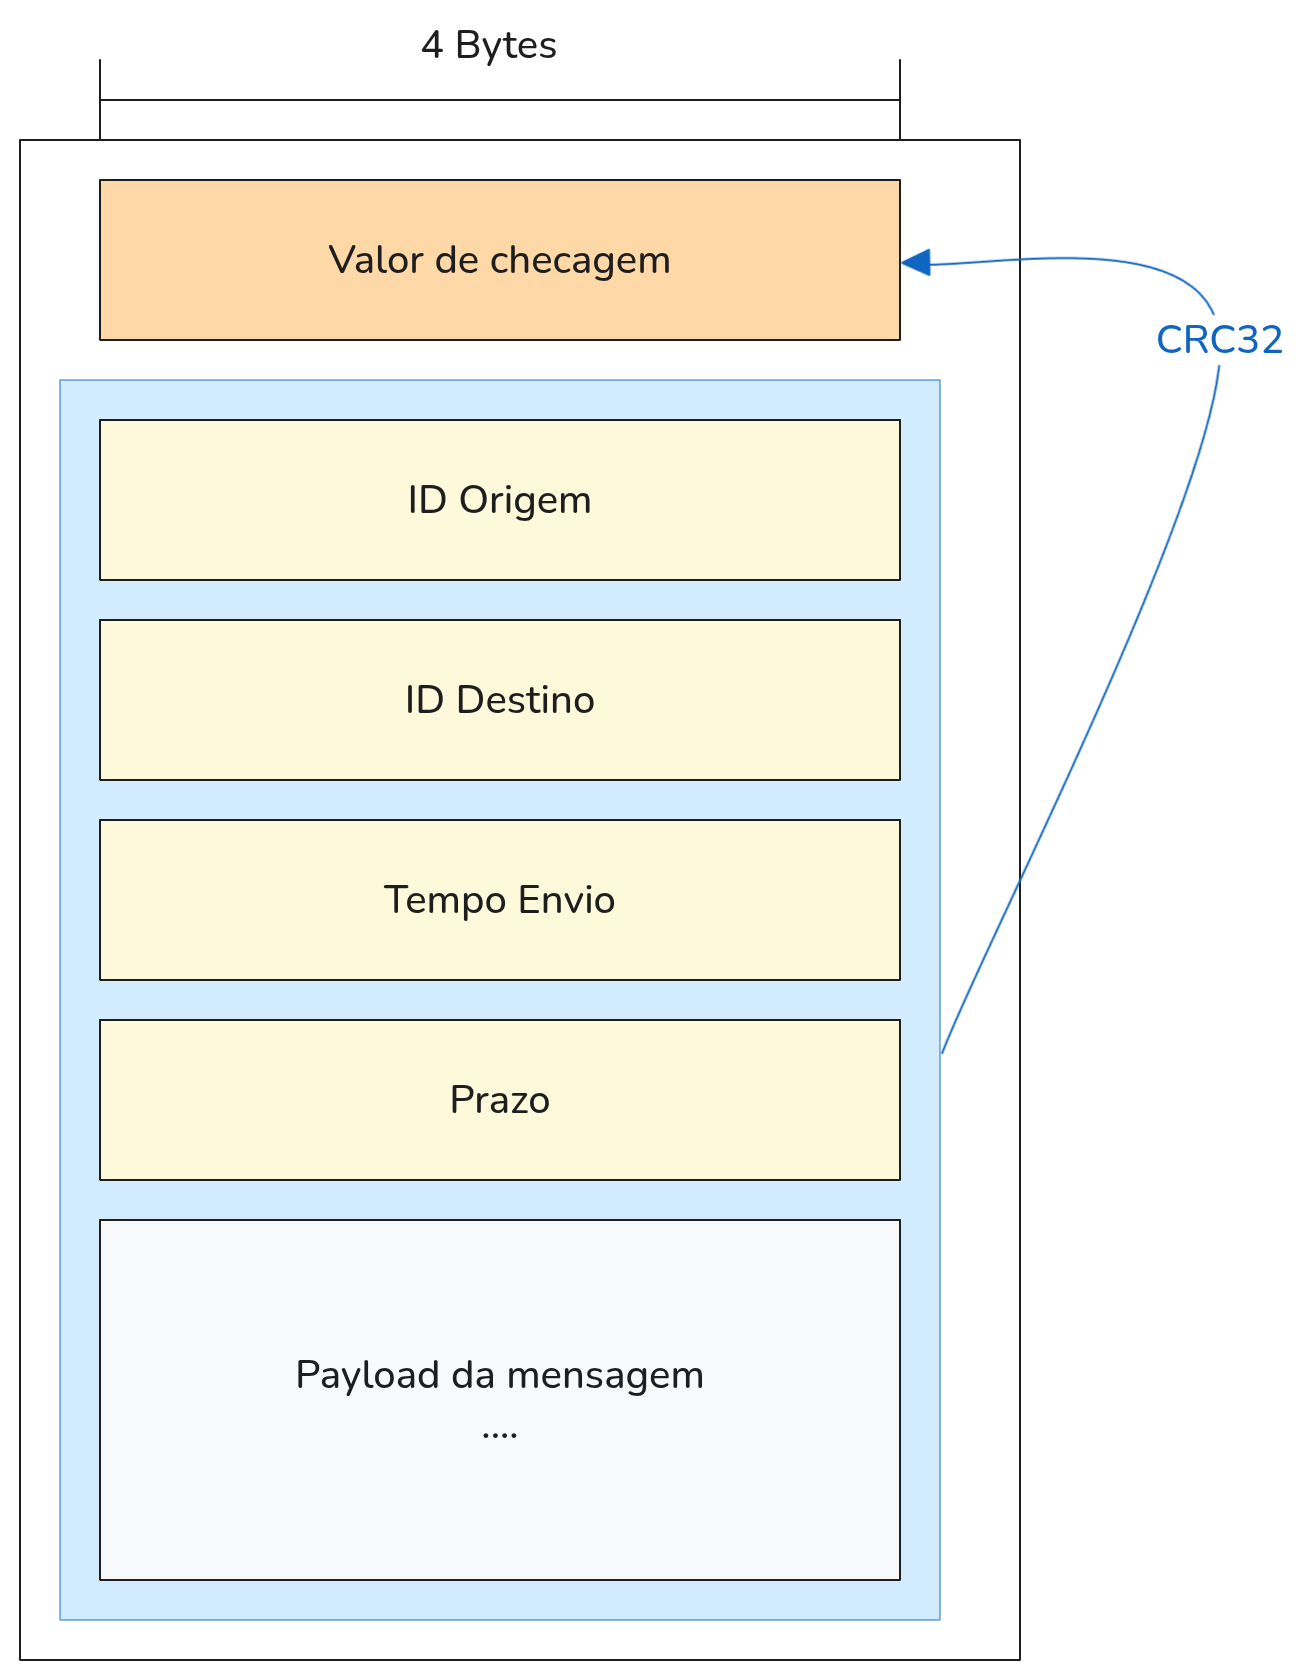
\includegraphics[width=0.50\textwidth]{assets/payload_layout.png}
    \captionsetup{justification=raggedright}
    \caption*{Fonte: Elaborada pelo autor}
    \label{fig:messageStruct}
\end{figure}

A tarefa é um objeto de interface que abstrai parte do estado utilizado pelo RTOS e provê métodos para sua inicialização, término e cancelamento. Uma tarefa possui um espaço de pilha dedicado, e uma V-Table que inclui os métodos providos para sua execução. A identificação da tarefa se dá pelo seu ID, que diretamente mapeia o recurso que encapsula o estado da tarefa no RTOS. O diagrama na \autoref{fig:bddTarefa} demonstra a relação de uma tarefa e os outros componentes do sistema.

\begin{figure}[H]
    \centering
    \captionsetup{justification=centering}
    \caption{Objeto que implementa a interface de Tarefa}
    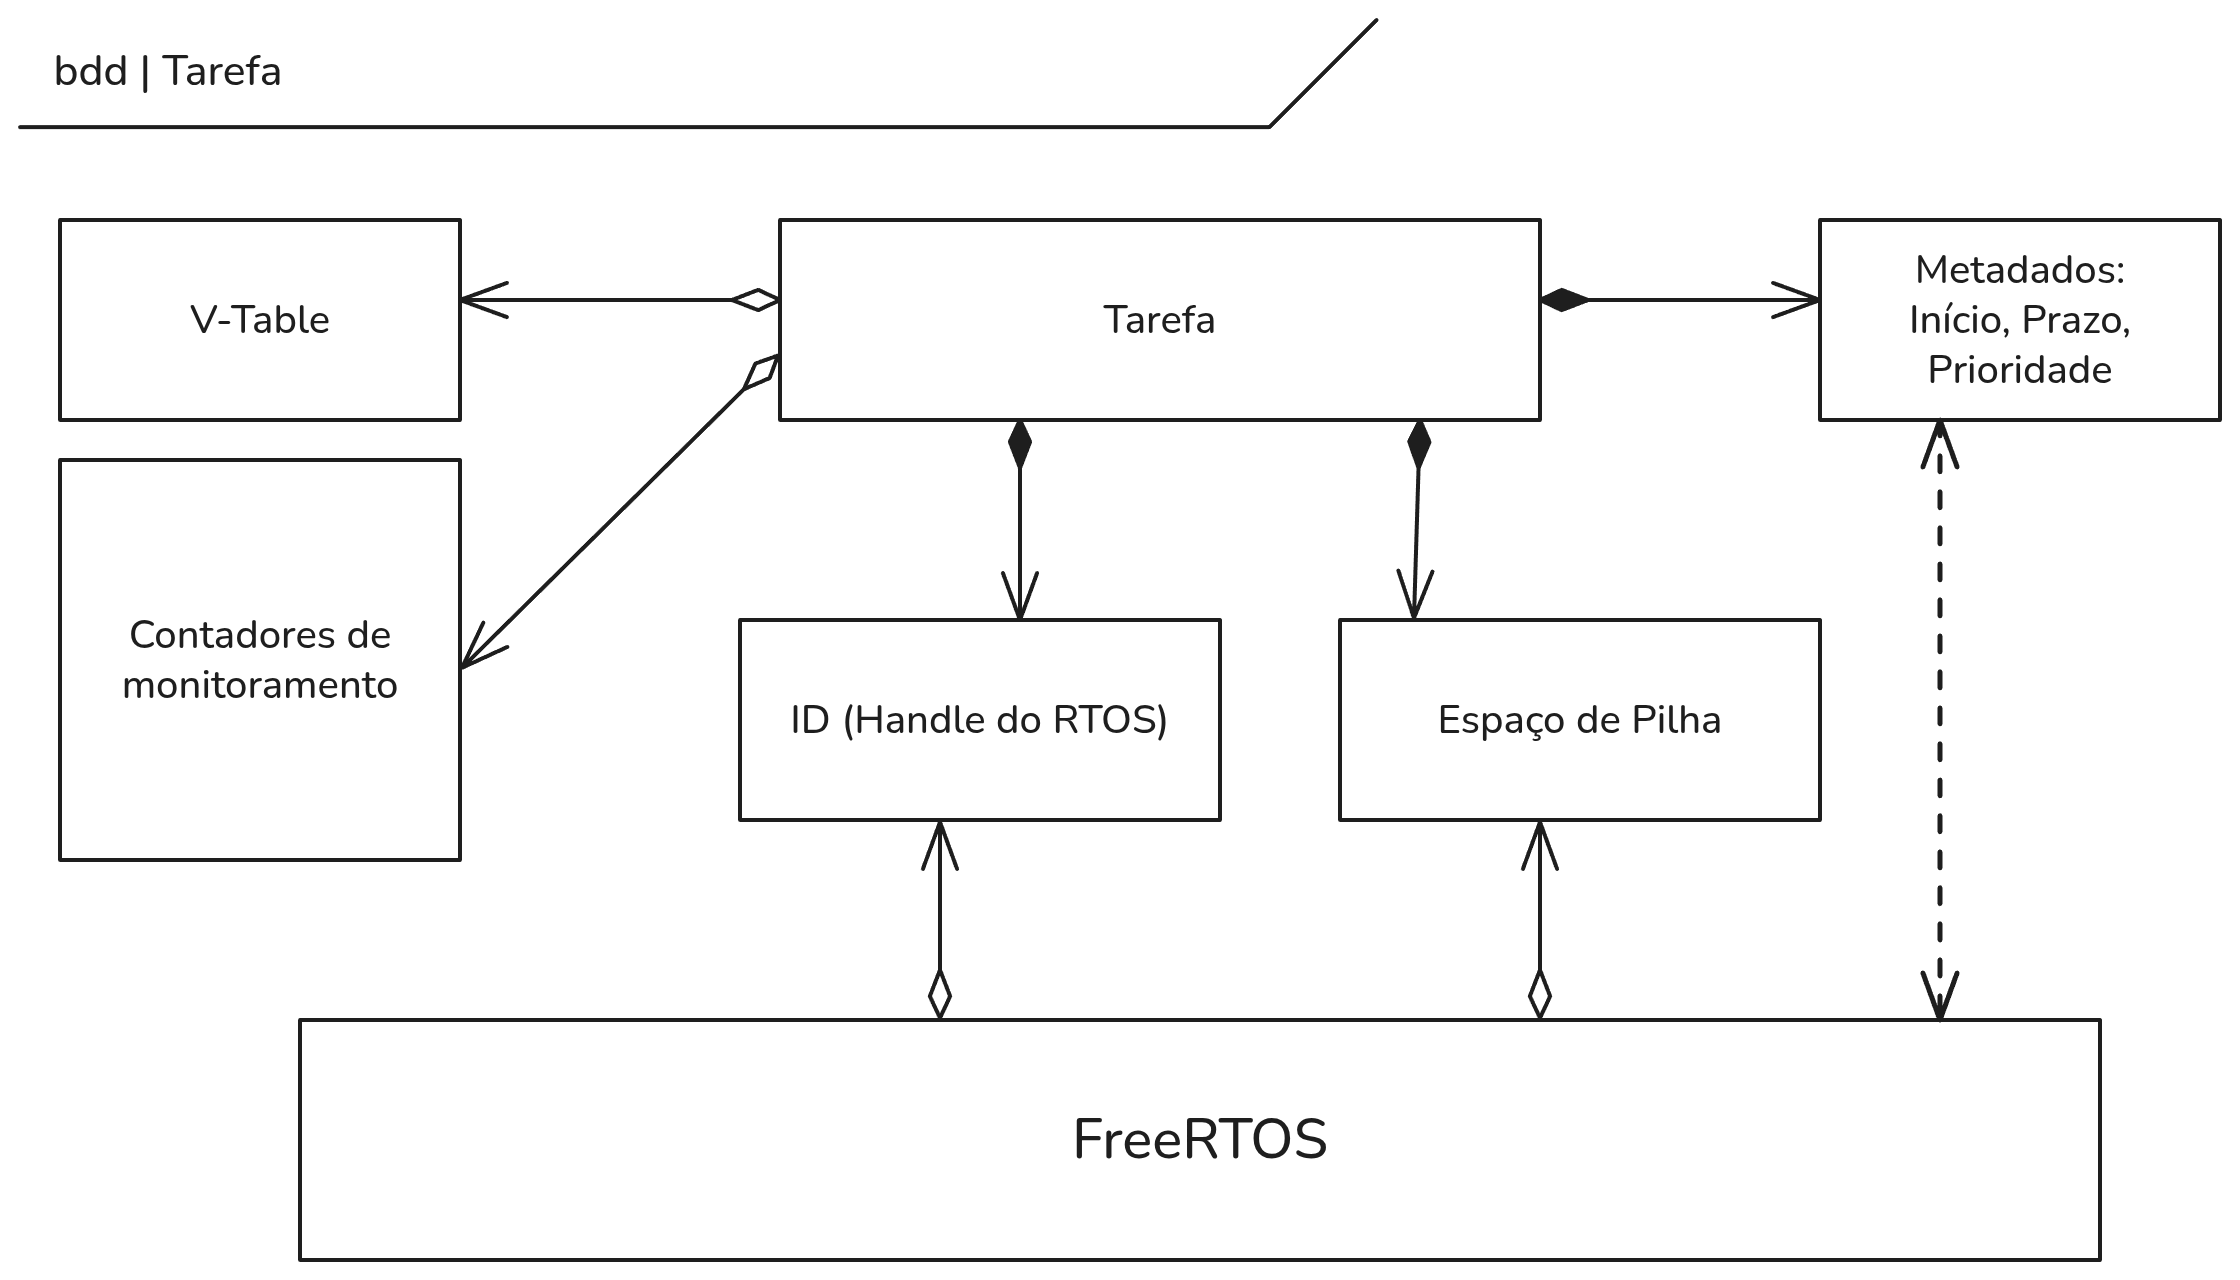
\includegraphics[width=0.90\textwidth]{assets/task_bdd.png}
    \captionsetup{justification=raggedright}
    \caption*{Fonte: Elaborada pelo autor}
    \label{fig:bddTarefa}
\end{figure}

A \autoref{fig:bddTarefa} omite a replicação da V-Table por clareza visual, mas antes da invocação de qualquer método da V-Table, será feito uma comparação adicional com outras duas tabelas redundantes para detectar corrupções na própria tabela durante a indireção por ponteiro de função.

\subsection{Algoritmos e Técnicas} \label{subsec:algoritmos}

Para a implementação da funcionalidade de tolerância à falhas, algumas das técnicas abordadas no \autoref{cap:fund} serão utilizadas. O detalhamento sobre a implementação será abordado nesta seção.

\subsubsection{CRC: Cyclic Redundancy Check}

Será implementado o CRC-32C, que já é aplicado em sistemas de arquivos como o Btrfs e o ext4, assim como em protocolos de rede como iSCSI e SCTP. Seu Polinômio geradador $P$ é:

\begin{equation}
    \begin{split}
        P = & x^{32} + x^{28} + x^{27} + x^{26} + x^{25} + x^{23} + x^{22} + x^{20} \\
            & + x^{19} + x^{18} + x^{14} + x^{13} + x^{11} + x^{10} + x^{9} + x^{8} + x^{6} + 1
    \end{split}
\end{equation}
\addEquacao{Polinômio CRC-32C}{5}


\subsubsection{Redundância Modular}

Para a aplicação da redundância modular, neste caso a redundância modular tripla, será feito a replicação concorrente da tarefa, cada tarefa possui um espaço de pilha próprio e são escalonadas de forma convencional pelo FreeRTOS. O corpo das tarefas não é replicado, e continua como parte de memória para apenas leitura e execução, um exemplo da relação de réplicas de tarefas executando em relação ao resto do sistema pode ser observado na \autoref{fig:bddTMR}.

\begin{figure}[H]
    \centering
    \captionsetup{justification=centering}
    \caption{Diagrama de bloco de Redundância modular}
    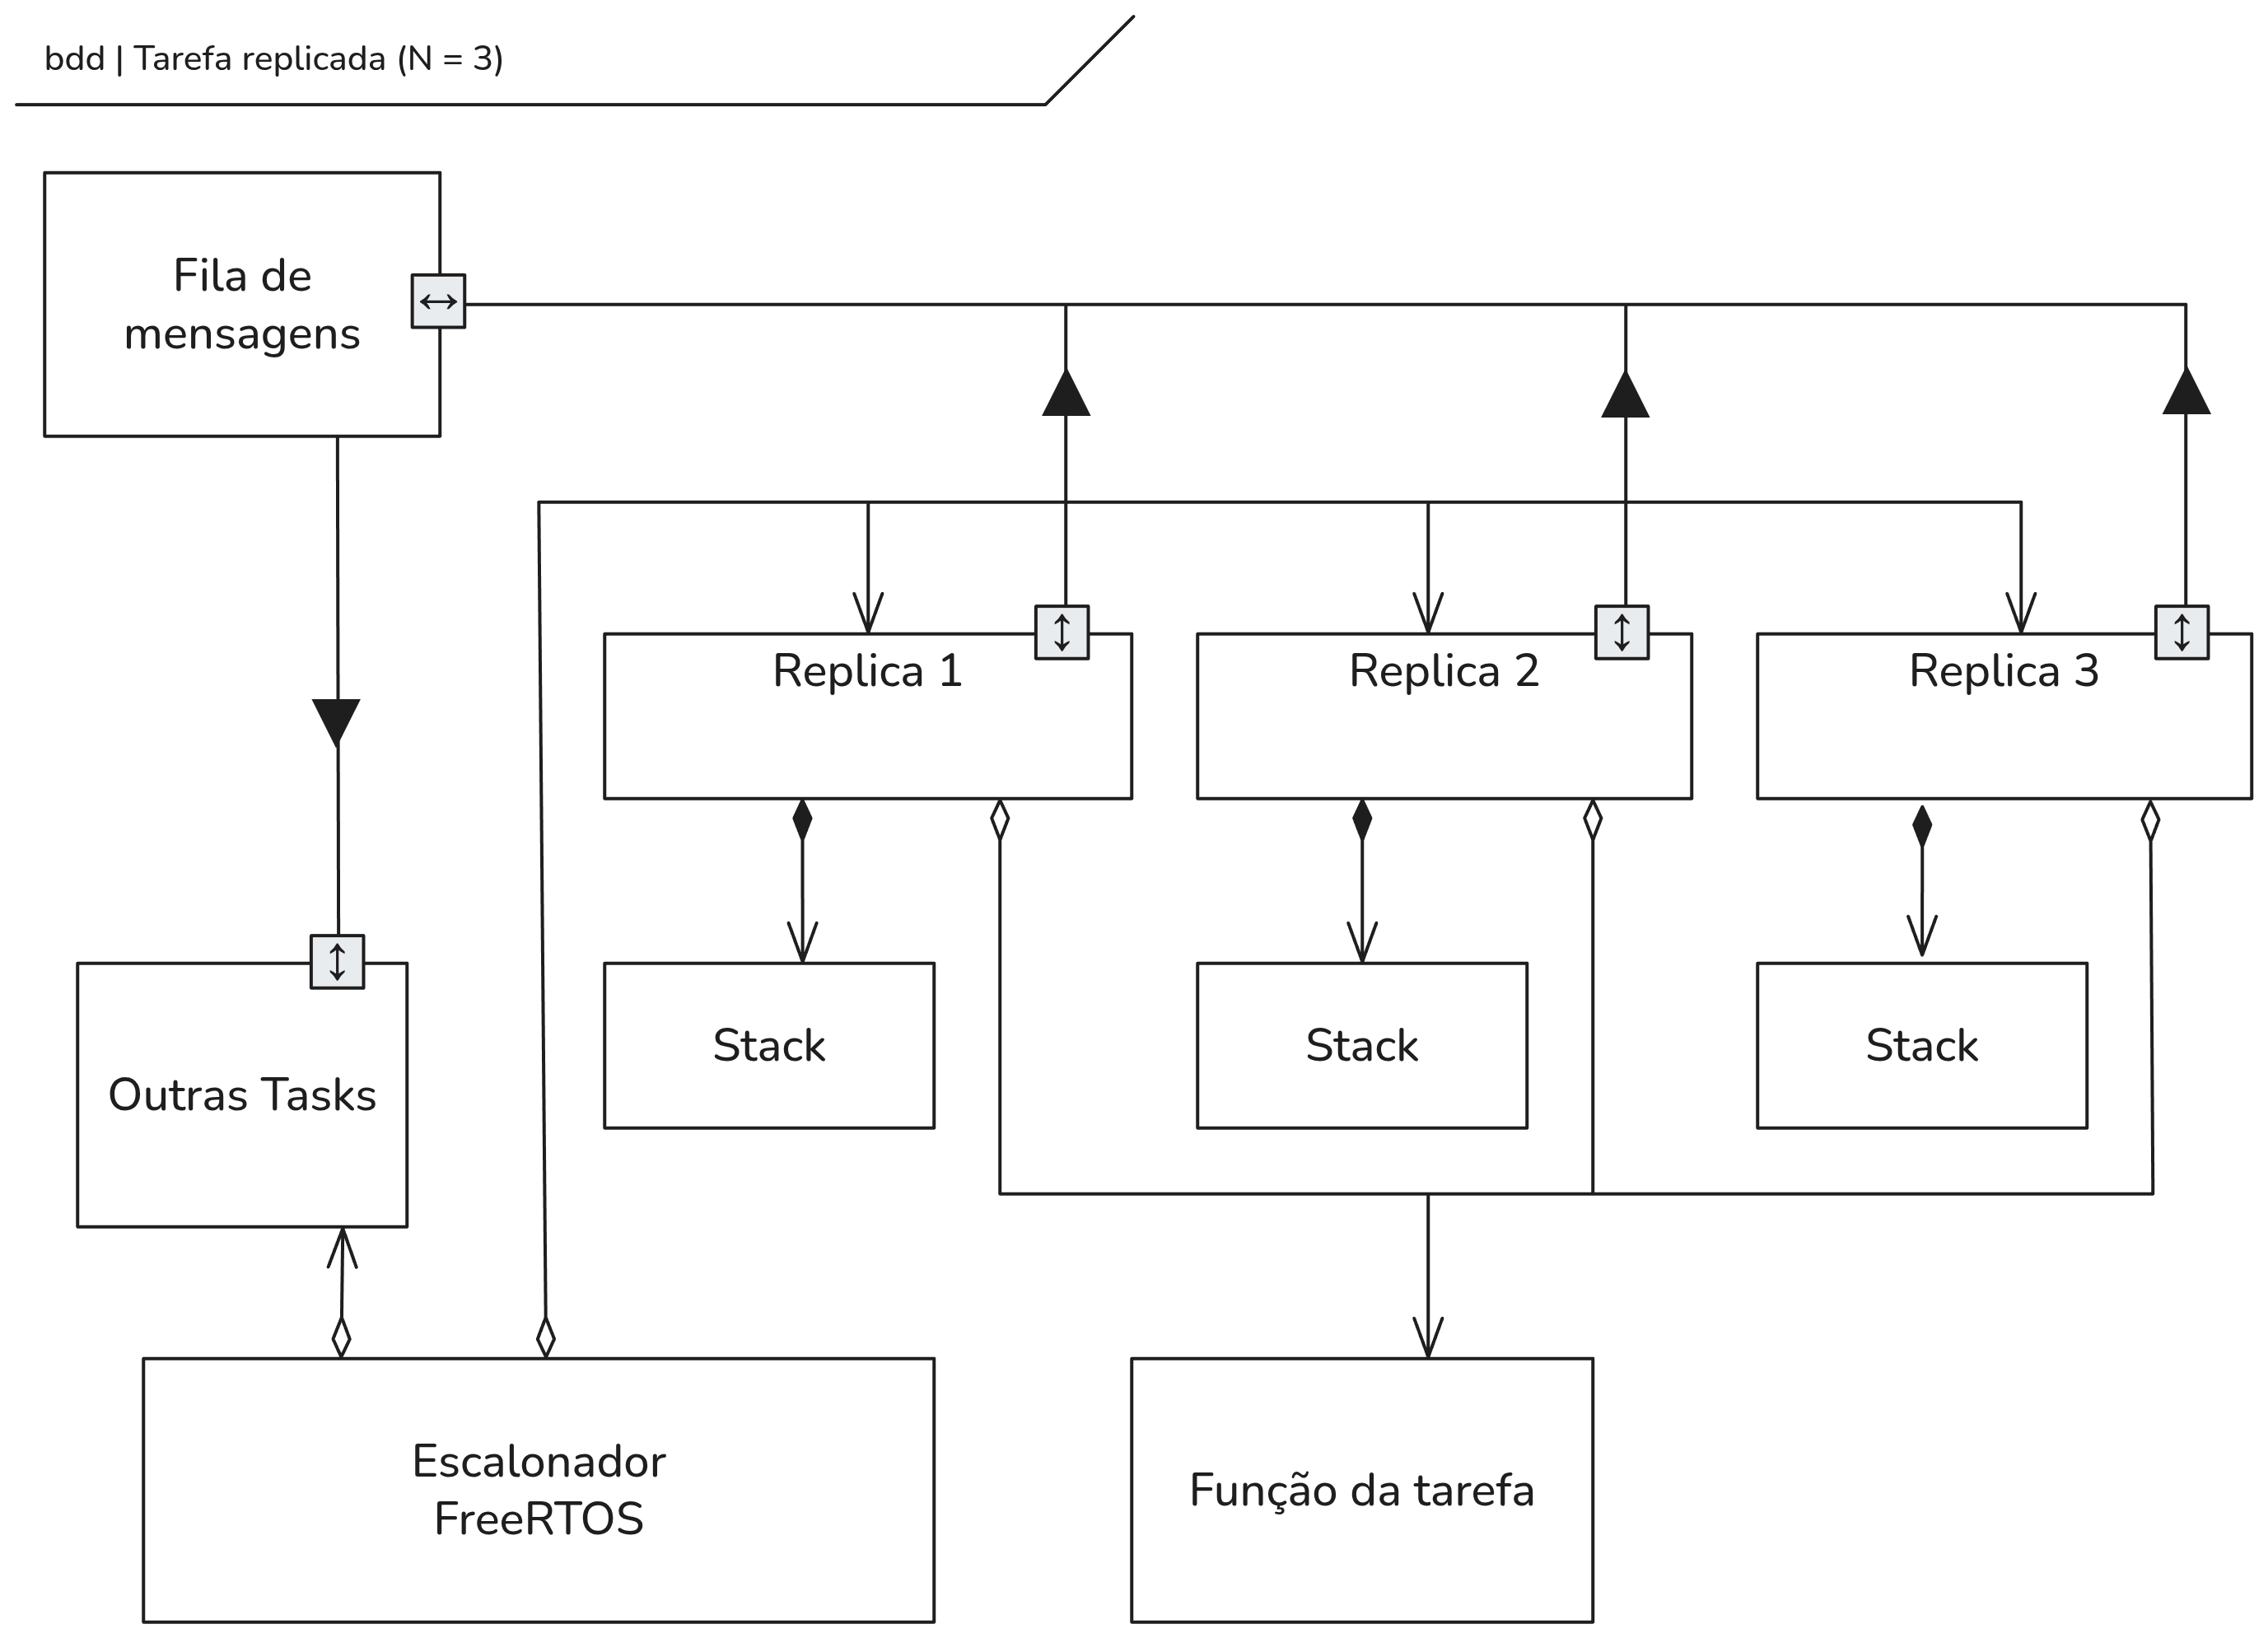
\includegraphics[width=0.950\textwidth]{assets/tmr_bdd.png}
    \captionsetup{justification=raggedright}
    \caption*{Fonte: Elaborada pelo autor}
    \label{fig:bddTMR}
\end{figure}

\subsubsection{Reexecução}

A implementação de tarefas com reexecução é baseada no uso de execuções consecutivas que reutilizam do mesmo espaço de pilha, uma tarefa pode ser sempre reexecutada $N$ vezes, servindo um propósito similar à técnica de redundância, ou executada \textit{até} $N$ vezes, encerrando a execução imediatamente após não encontrar nenhuma falha. Para os propósitos deste trabalho, será utilizada a segunda técnica, pois permite mais oportunidade para o escalonador encaixar trabalho no tempo ocioso, e também por ser um exemplo mais bem estudado na fundamentação teórica deste trabalho por Isosimov et. al.

Assumindo $N = 3$, o diagrama na \autoref{fig:stateReexec} descreve uma máquina de estado finito para a execução de uma tarefa com reexecução, espera-se que o caso médio seja a execução diretamente para um estado correto. Para a criação de uma condição de transparência, o prazo da tarefa deve ser o pior caso possível de $N$ execuções.

\begin{figure}[H]
    \centering
    \captionsetup{justification=centering}
    \caption{Estados de uma reexecução}
    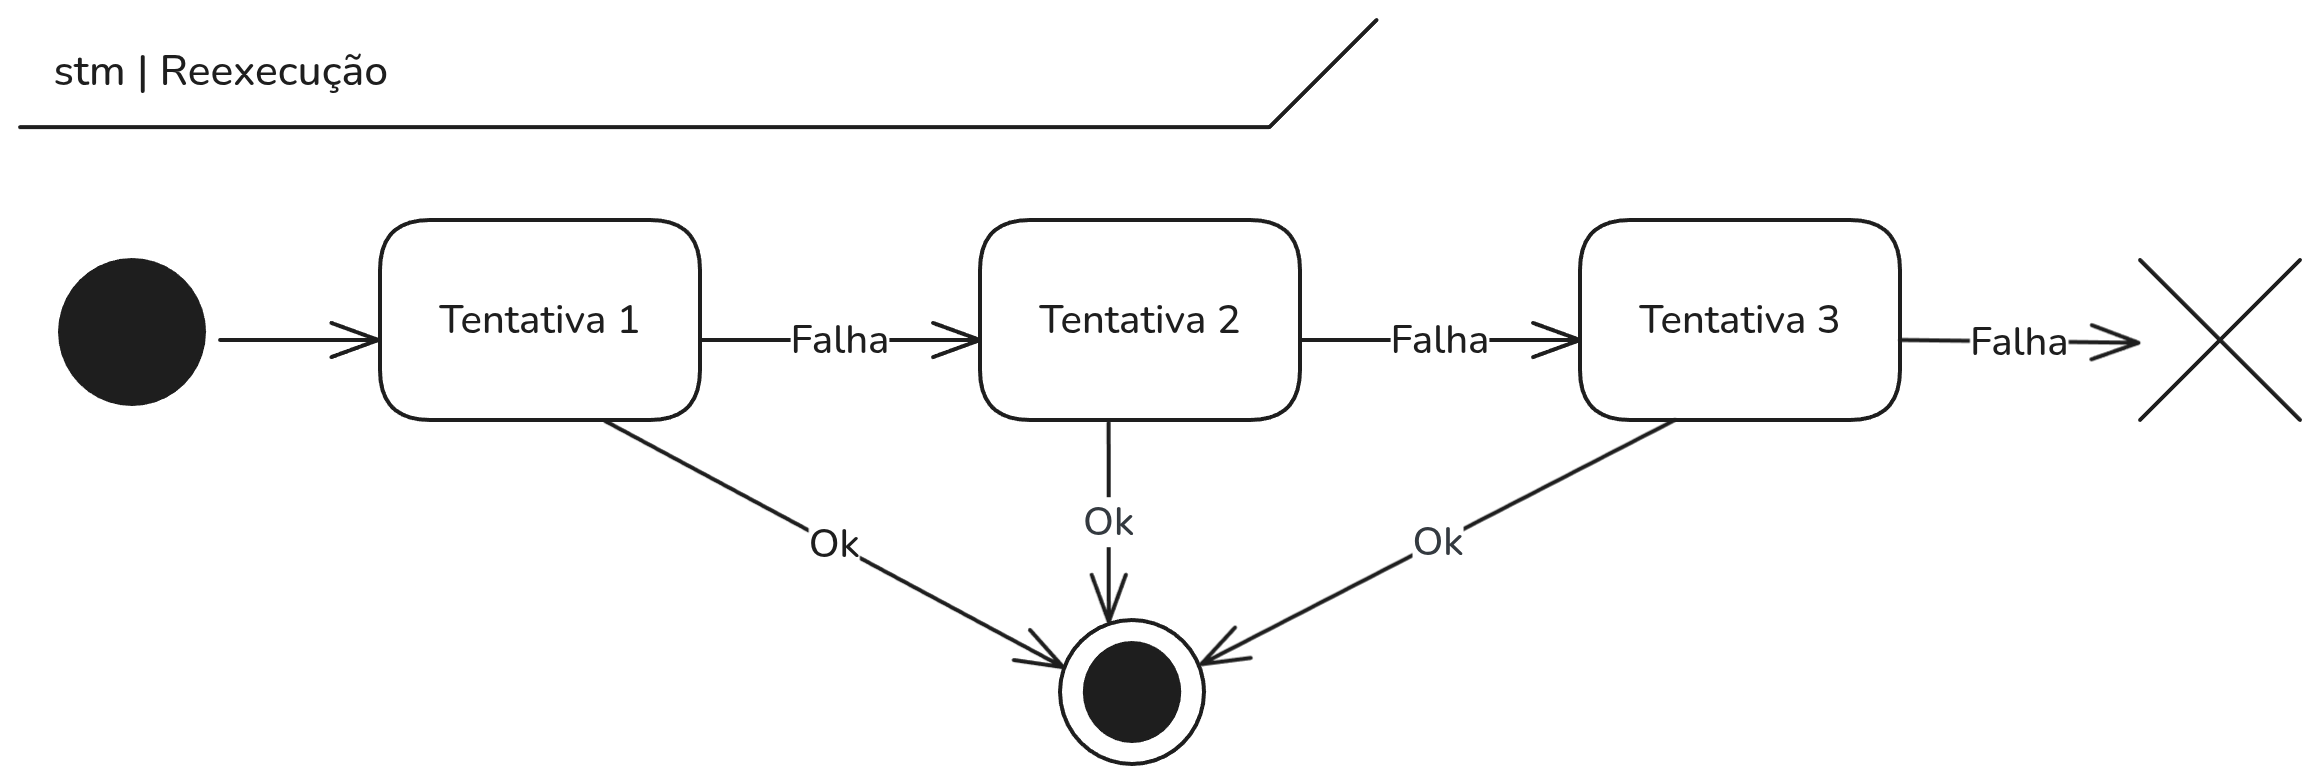
\includegraphics[width=0.925\textwidth]{assets/state_reexec.png}
    \captionsetup{justification=raggedright}
    \caption*{Fonte: Elaborada pelo autor}
    \label{fig:stateReexec}
\end{figure}

\subsubsection{Sinal Heartbeat}

Para a implementação dos sinais de heartbeat será utilizado uma tarefa que servirá como um monitor que associa os IDs de outras tarefas com um timer de sinal, o sinal será propagado com escrita atômica de um número e o temporizador do sistema no momento da escrita, se houver uma violação do prazo combinado na criação da tarefa e o prazo apresentado, é considerado que ocorreu uma falha. Este fluxo é visualmente representado na \autoref{fig:heartbeatAdv}. Essa técnica pode ser utilizada para cancelar tarefas presas no caso de replicação assim como iniciar uma reexecução antecipada.

\begin{figure}[H]
    \centering
    \captionsetup{justification=centering}
    \caption{Estados de uma reexecução}
    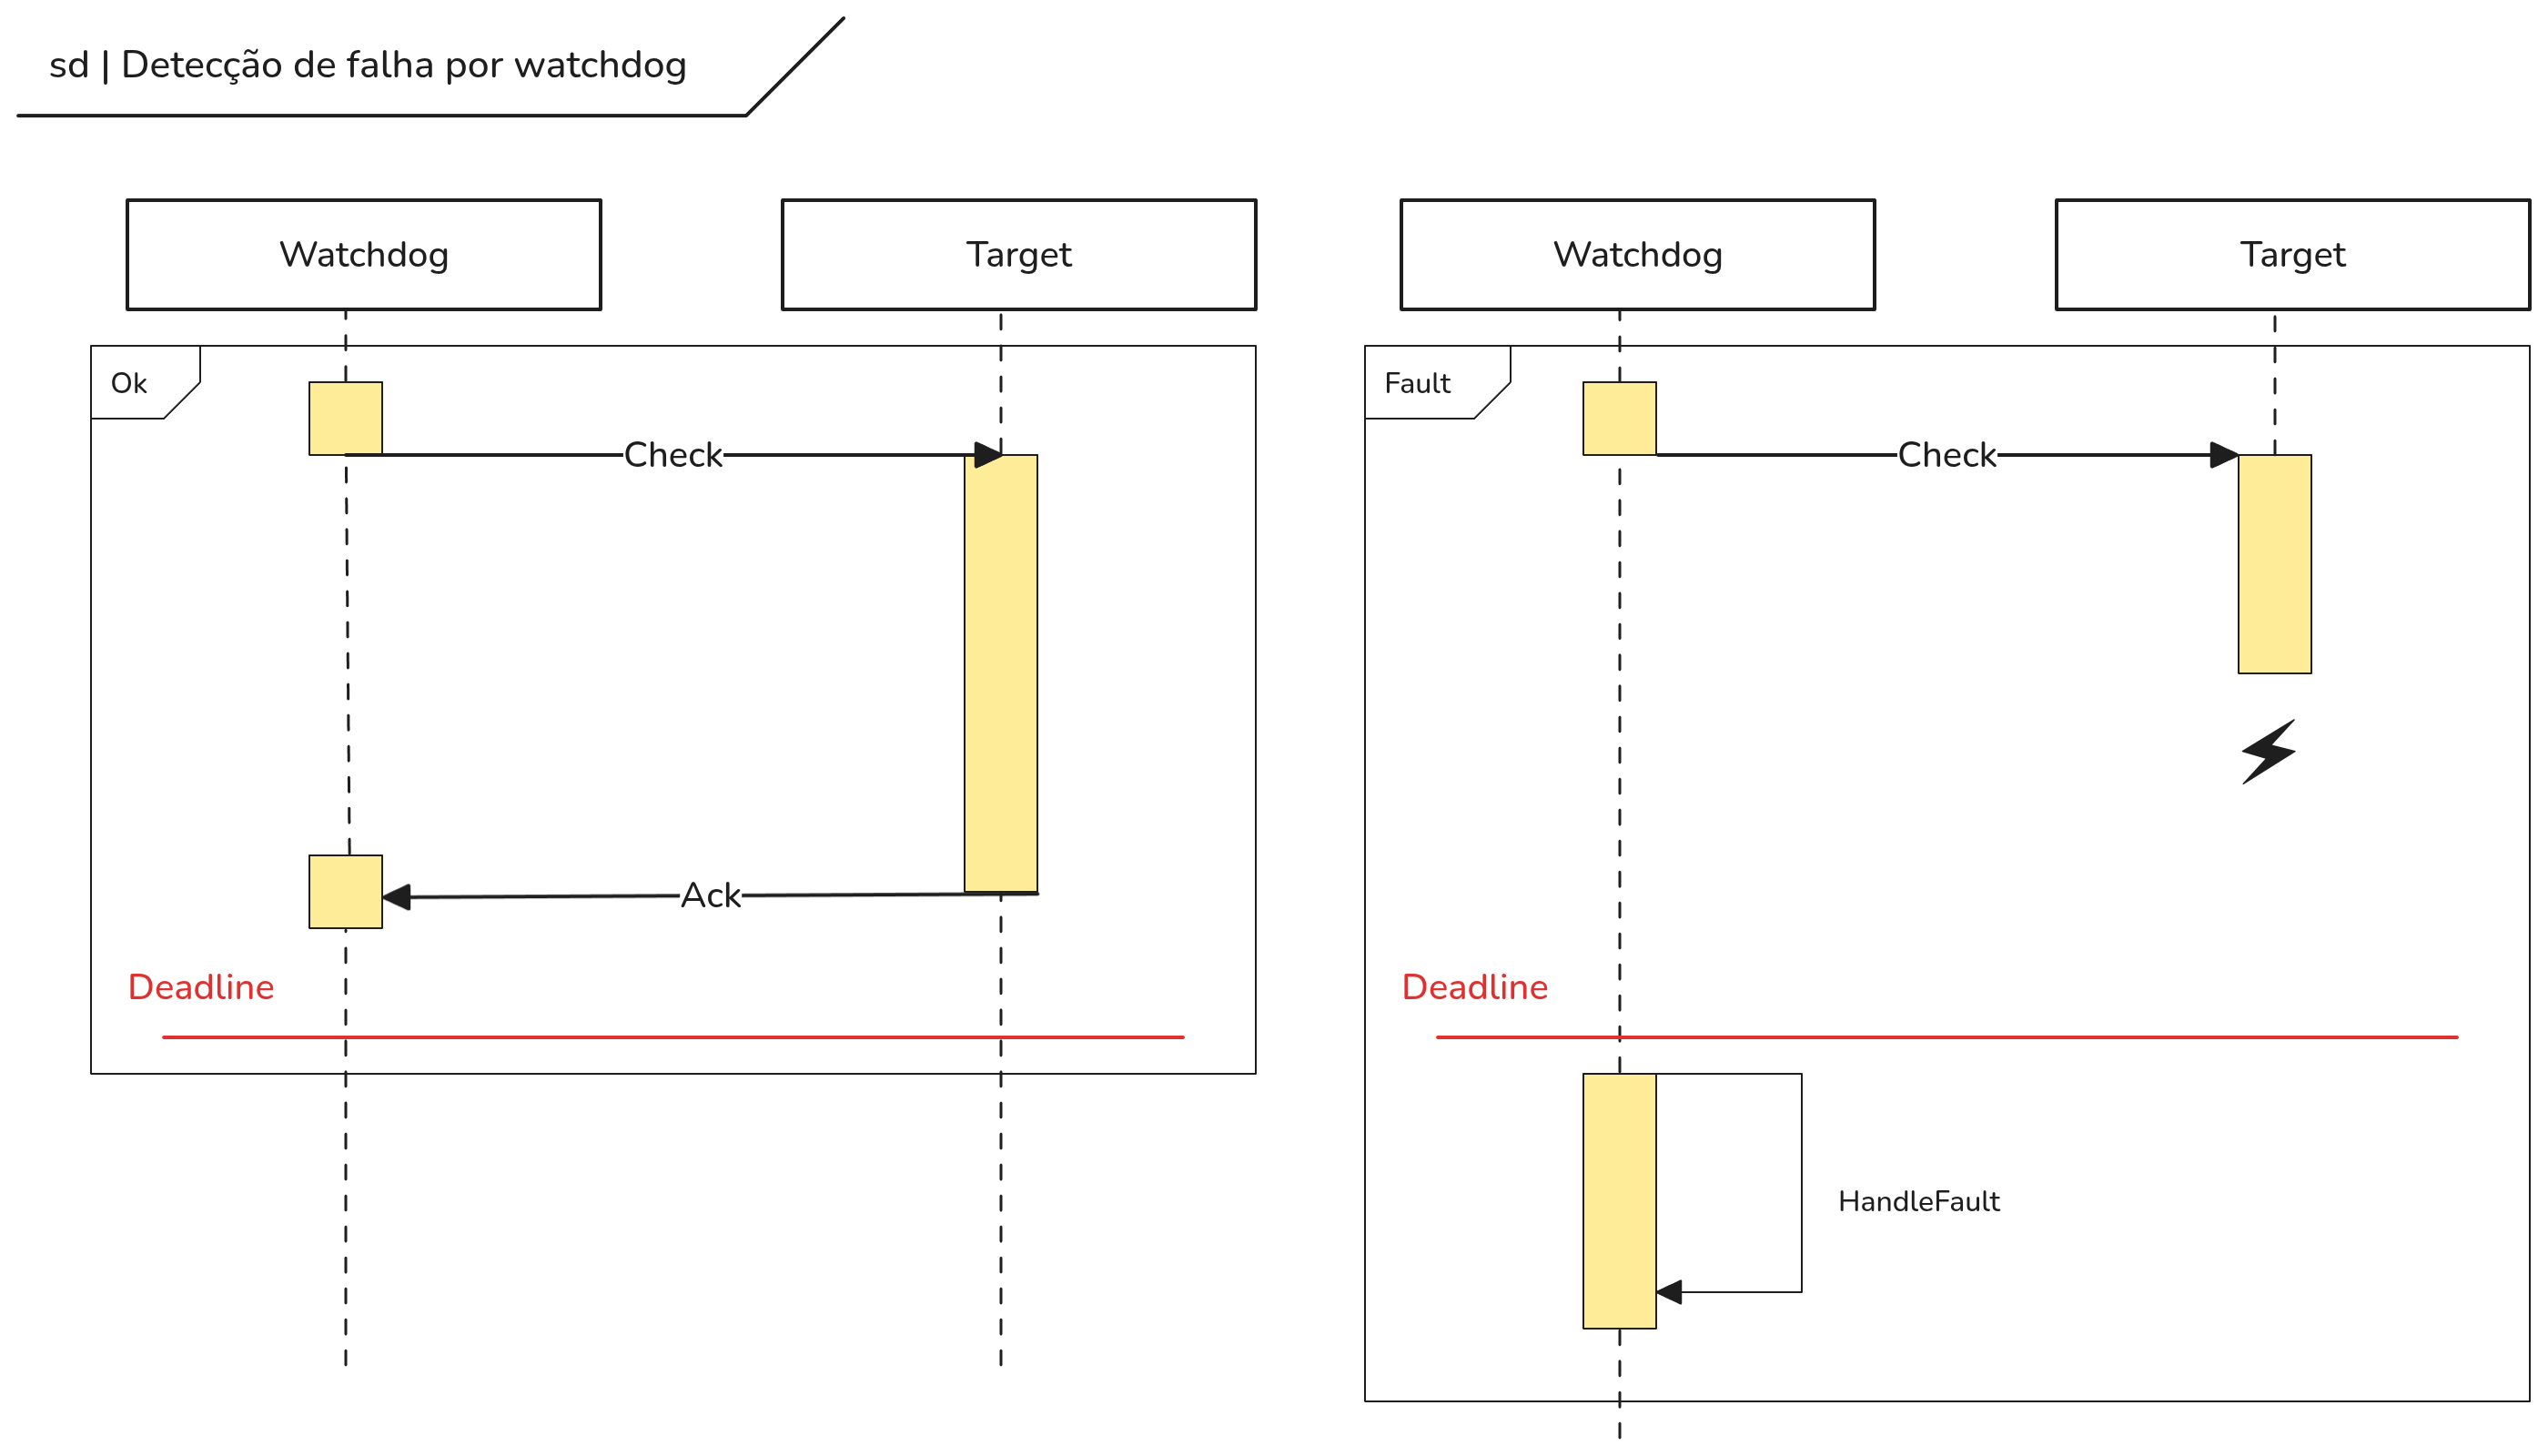
\includegraphics[width=0.95\textwidth]{assets/heartbeat_signal.png} %TODO: Imagem melhor
    \captionsetup{justification=raggedright}
    \caption*{Fonte: Elaborada pelo autor}
    \label{fig:heartbeatAdv}
\end{figure}

\subsubsection{Asserts}

Asserts serão utilizados para verificar invariantes, qualquer quebra de contrato de função ou invariante que é coberta com um assert deve resultar em uma falha.

\section{Plano de Verificação}

Para a validação dos algoritmos e técnicas utilizadas(\textbf{RF01}, \textbf{RF07}) será feito uma série de testes unitários e de integração, para garantir que as técnicas estejam ao menos corretamente implementadas antes de realizar qualquer tipo de medição.

A validação da detecção de falhas e vencimento de prazos (\textbf{RF05}, \textbf{RF06}) serão preliminarmente testadas com injeção lógica em software utilizando o emulador QEMU com a mesma arquitetura de processador executando o sistema FreeRTOS e será validado definitivamente durante o teste com injeção lógica em hardware. A capacidade de criar, destruir e cancelar tarefas (\textbf{RF02}) é um pré-requisito e será verificada com um simples teste ponta a ponta. Importante notar que a priorização de tarefas baseadas em seu número de prioridade e parte dos algoritmos de comunicação entre tarefas já são implementados no FreeRTOS.

Como o produto final do trabalho requer uma análise de resiliência e do custo das técnicas, a seção seguinte aborda a campanha de injeção utilizada, que será aplicada com método lógico em hardware para a análise final.

\subsection{Campanha de Injeção de Falhas} \label{subsec:campanhaInjecao}

Para testar a injeção de falhas serão utilizados mecanismos lógicos em software e em hardware com com o auxílio do depurador ST-Link. As falhas serão de natureza transiente e focarão no segmento de memória com leitura e escrita.

As falhas injetadas serão falhas transientes de memória onde $N$ bytes a partir de um endereço base são escolhidos e invertidos com um XOR de uma mascara aleatória, as regiões de memória escolhidas serão o segmento estático com escrita, a pilha das tarefas e registradores de propósito geral. Os programas exemplo serão executados por um número fixo de rodadas (e.x: 200) e terão suas métricas coletadas e catalogadas para análise posterior.

Falhas detectadas serão armazenadas com contadores atômicos, com um contador dedicado para cada tipo de técnica. A região de coleta das métricas será reservada previamente na seção estática da imagem do executável e será isenta de falhas.

Para os testes, as combinações de técnicas escolhidas foram: nenhuma técnica como grupo de controle, técnicas simples (CRC e Asserts) que não interferem na execução e combinações de técnicas que alteram o fluxo do programa (Reexecução e Replicação) com e sem validação de prazo via sinal heartbeat. As combinações estão listadas no \autoref{tab:combinacoesTecnicas}.

\begin{quadro}[H]
    \centering
    \caption{Combinações de técnicas utilizadas}
    \begin{tabular}{|c|c|c|c|c|}
        \hline
        \rowcolor[HTML]{C0C0C0}
        \textbf{Reexecução} & \textbf{Redundância modular} & \textbf{Heartbeat Signal} & \textbf{CRC} & \textbf{Asserts} \\
        \hline
        - & - & - & - & - \\
        \hline
        - & - & - & X & X \\
        \hline
        X & - & - & X & X \\
        \hline
        X & - & X & X & X \\
        \hline
        - & X & - & X & X \\
        \hline
        - & X & X & X & X \\
        \hline
    \end{tabular}
    \label{tab:combinacoesTecnicas}
\end{quadro}

\subsection{Programas de Teste}

Para testar a viabilidade e o impacto das técnicas implementadas, serão desenvolvidas duas aplicações pequenas para testes. A primeira realizará um filtro passa-banda com no domínio da frequência (necessitando de uma transformada de Fourier) de uma onda fornecida como entrada, o processamento será feito em lotes. Já o segundo programa realizará uma convolução bidimensional para aplicar um filtro Laplaciano.

A escolha da primeira aplicação serve primariamente testar uma operação que dependa de múltiplos acessos e modificações à memória e que possa demonstrar capacidades de processamento assíncronas (padrão produtor/consumidor), que são particularmente importantes ao se lidar com múltiplas interrupções causadas por temporizadores ou IO.

Já o segundo programa, de natureza mais simples, visa causar alto estresse em termos de leituras, juntamente com muitas operações aritméticas, mas com menos ênfase em comunicação entre tarefas. O objetivo é testar o impacto das técnicas em um caso mais extremo que requer muito processamento.

Ambos os programas são problemas que requerem um uso de CPU relativamente alto, o que pode auxiliar a notar violações do critério de tempo real ou uma variação muito grande no tempo de execução, que não é muito desejada mesmo que cumpra o prazo. As implementações dos algoritmos para estes programas são primariamente extraídos de um livro de processamento digital de sinais por \citeindirect{GuideToDSP}.

\section{Análise de Riscos} \label{sec:analiseRiscos}

O trabalho é de risco baixo, dado que constrói em cima de fundações técnicas previamente exploradas, porém dentro dos principais riscos que possam alterar ou causar problemas durante a produção da análise encontram-se:

\begin{quadro}[H]
    \centering
    \caption{Análise de riscos}
    \begin{tabular}{|p{0.20\textwidth}|p{0.150\textwidth}|p{0.10\textwidth}|p{0.20\textwidth}|p{0.20\textwidth}|}
        \hline
        \rowcolor[HTML]{C0C0C0}
        \textbf{Risco} & \textbf{Probabilidade} & \textbf{Impacto} & \textbf{Gatilho} & \textbf{Mitigação} \\
        \hline

        Funcionalidades e API do RTOS é incompatível com a interface proposta pelo trabalho &  Baixo & Alto & Implementar interface no RTOS & Utilizar outro RTOS, modificar o FreeRTOS, adaptar a interface \\
        \hline

        Problemas para injetar falhas com depurador em hardware & Baixa & Alto & Realizar injeção no microcontrolador & Utilizar de outro depurador, depender de falhas lógicas em software como última alternativa \\
        \hline

        Não conseguir coletar métricas de performance com profiler do FreeRTOS & Baixa & Médio & Teste em microcontrolador ou ambiente virtualizado & Inserir pontos de medição manualmente \\
        \hline
    \end{tabular}
    \label{tab:riscos}
\end{quadro}

\section{Cronograma do TCC3}

\begin{quadro}[H]
    \centering
    \caption{Combinações de técnicas utilizadas}
    \begin{tabular}{|p{0.25\textwidth}|c|c|c|c|c|c|c|}
    \hline
    \rowcolor[HTML]{C0C0C0}
    \hline
    \textbf{Atividade} & \textbf{07/2025} & \textbf{08/2025} & \textbf{09/2025} & \textbf{10/2025} & \textbf{11/2025} & \textbf{12/2025} \\
    \hline
    Escrita da Monografia                           & XXXX & XXXX & XXXX & XXXX  & XX-- & ---- \\
    \hline
    Implementação dos Algoritmos                    & XXXX & XX-- & ---- & ----  & ---- & ---- \\
    \hline
    Testes dos Algoritmos                           & XXXX & XX-- & ---- & ----  & ---- & ---- \\
    \hline
    Implementação dos Programas Exemplo             & ---- & --XX & XXX- & ----  & ---- & ---- \\
    \hline
    Teste dos Programas Exemplo                     & ---- & --XX & XXX- & ----  & ---- & ---- \\
    \hline
    Implementação da Injeção com Hardware           & ---- & ---- & -XXX & XX--  & ---- & ---- \\
    \hline
    Execução microcontrolador e coleta das métricas & ---- & ---- & ---- & XXXX  & X--- & ---- \\
    \hline
    Revisão Textual                                 & ---- & ---- & ---- & --XX  & XXXX & XX-- \\
    \hline
    \end{tabular}
    \label{tab:riscos}
\end{quadro}


  % table.header([*Atividade*], [*07/2025*], [*08/2025*], [*09/2025*], [*10/2025*], [*11/2025*], [*12/2025*]),
  % [Escrita da Monografia],                           [`XXXX`], [`XXXX`], [`XXXX`], [`XXXX`],  [`XXXX`], [`X___`],
  % [Implementação dos Algoritmos],                    [`XXXX`], [`XX__`], [`____`], [`____`],  [`____`], [`____`],
  % [Testes dos Algoritmos],                           [`XXXX`], [`XX__`], [`____`], [`____`],  [`____`], [`____`],
  % [Implementação dos Programas Exemplo],             [`____`], [`__XX`], [`XXX_`], [`____`],  [`____`], [`____`],
  % [Teste dos Programas Exemplo],                     [`____`], [`__XX`], [`XXX_`], [`____`],  [`____`], [`____`],
  % [Implementação da Injeção com Software],           [`____`], [`____`], [`XXXX`], [`____`],  [`____`], [`____`],
  % [Implementação da Injeção com Hardware],           [`____`], [`____`], [`__XX`], [`XXX_`],  [`____`], [`____`],
  % [Execução microcontrolador e coleta das métricas], [`____`], [`____`], [`____`], [`__XX`],  [`XXXX`], [`____`],
  % [Revisão Textual],                                 [`____`], [`____`], [`____`], [`____`],  [`__XX`], [`XXXX`],


% -- TODO ---
% Novo digrama pro heartbeat signal

% Comentários Douglas
%  - Rever os objetivos específicos e geral para deixar mais explicativo e fechar melhor o escopo
%  - Materiais antes de métodos
%  - Trabalhos relacionados pode ser melhor explorados
%  - Fraco refereciamento em vários itens do texto
%  - Muitas palavras em inglês
%  - Melhorar requisito funcionais
%  - Falta um texto de suporte do visão geral
%  - Faltam diagramas para suportar a implementação (e não dos testes) junto ou talvez substituir trechos de código

% Comentários Tiago
%  - Destacar melhor características de tempo real: se não injetar nenhuma falta o seu sistema pode falhar?
%  - Destacar que o sistema é de tempo real e qual é o requisito de tempo real
%  - heartbit talvez seja a técnica para atrelar em teste de atender o requisito de tempo real.
%  - Plano de teste alinhados com os requisitos
%  - Diagramas de sequência (ou fluxograma) entre outros para descrever os testes 
%  - Analisar cronograma para realizar os testes

 \clearpage
\chapter{Considerações Finais}
\label{cap:consid}

Durante a pesquisa bibliográfica, foi possível observar uma variedade de técnicas de tolerância à falhas em software. Das técnicas escolhidas, optou-se por focar em técnicas mais simples para a detecção (CRC e Asserts), técnicas de execução que possibilitem a criação de condições de transparência (Replicação e Reexecução) e validação de prazos (Sinais Heartbeat).

O projeto de pesquisa visa avaliar a aplicação destas técnicas em um contexto de um sistema operacional de tempo real, utilizando de injeção de falhas lógicas em hardware para a construção de uma análise do impacto de diferentes combinações de técnicas. Algumas das hipóteses levantadas foram:

\begin{enumerate}
    \item Asserts terão um impacto pequeno na performance.
    \item Replicação de tarefas introduzirá maior variância no tempo de execução.
    \item Reexecução terá uma variância menor do que a replicação, porém com maior custo de tempo.
    \item Sinais de heartbeat terão um impacto menor na detecção de erros em relação à outras técnicas.
\end{enumerate}

Ao realizar uma análise do impacto das técnicas apresentadas espera-se melhor esclarecer quais trocas são realizadas ao escolher uma técnica de tolerância em software.
 \clearpage
% TCC 3
% \input{4_desenvolvimento} \clearpage
% \input{5_resultados} \clearpage
% \input{6_consideracoes} \clearpage

\postextual
\bibliography{refs.bib}  \clearpage

\end{document}
